\documentclass[12pt,a4paper]{article}

\usepackage[rmargin=1.2in,lmargin=1.2in,tmargin=.8in,bmargin=.8in]{geometry}
\usepackage{indentfirst}

% fonts
% \usepackage{mathptmx}
\usepackage{fontspec}
\setmainfont{Times New Roman}

% images, table and colors
\usepackage[dvipsnames]{xcolor}
\usepackage{graphicx,overpic} 
\graphicspath{ {./figures/}} 
\usepackage{wrapfig}

\usepackage{tabularx, makecell, booktabs}
\usepackage{caption}
\usepackage{enumitem}
\usepackage[normalem]{ulem}

% math support
\usepackage{amsmath}
\usepackage{amssymb}
\usepackage{siunitx}
\usepackage[version=4]{mhchem}

% for code display
\usepackage{minted}

% citations
\usepackage[colorlinks=true,allcolors=blue]{hyperref}
\usepackage[backend=biber,citestyle=authoryear-icomp,bibstyle=authoryear,hyperref=true,isbn=false,url=false,eprint=false,date=year,maxcitenames=2,giveninits=true,uniquename=init,uniquelist=minyear,sorting=nyt]{biblatex}
\DeclareNameAlias{default}{family-given}
\DeclareNameAlias{sortname}{family-given}
\addbibresource{./pdr_references.bib}
%
%  These Macros are taken from the AAS TeX macro package version 5.2
%  and are compatible with the macros in the A&A document class
%  version 7.0
%  Include this file in your LaTeX source only if you are not using
%  the AAS TeX macro package or the A&A document class and need to
%  resolve the macro definitions in the TeX/BibTeX entries returned by
%  the ADS abstract service.
%
%  If you plan not to use this file to resolve the journal macros
%  rather than the whole AAS TeX macro package, you should save the
%  file as ``aas_macros.sty'' and then include it in your LaTeX paper
%  by using a construct such as:
%	\documentstyle[11pt,aas_macros]{article}
%
%  For more information on the AASTeX and A&A packages, please see:
%       http://journals.aas.org/authors/aastex.html	
%       ftp://ftp.edpsciences.org/pub/aa/readme.html
%  For more information about ADS abstract server, please see:
%       http://adsabs.harvard.edu/ads_abstracts.html
%

% Abbreviations for journals.  The object here is to provide authors
% with convenient shorthands for the most "popular" (often-cited)
% journals; the author can use these markup tags without being concerned
% about the exact form of the journal abbreviation, or its formatting.
% It is up to the keeper of the macros to make sure the macros expand
% to the proper text.  If macro package writers agree to all use the
% same TeX command name, authors only have to remember one thing, and
% the style file will take care of editorial preferences.  This also
% applies when a single journal decides to revamp its abbreviating
% scheme, as happened with the ApJ (Abt 1991).

\makeatletter
\let\jnl@style=\rm
\def\ref@jnl#1{{\jnl@style#1}}

\def\aj{\ref@jnl{AJ}}                   % Astronomical Journal
\def\actaa{\ref@jnl{Acta Astron.}}      % Acta Astronomica
\def\araa{\ref@jnl{ARA\&A}}             % Annual Review of Astron and Astrophys
\def\apj{\ref@jnl{ApJ}}                 % Astrophysical Journal
\def\apjl{\ref@jnl{ApJ}}                % Astrophysical Journal, Letters
\def\apjs{\ref@jnl{ApJS}}               % Astrophysical Journal, Supplement
\def\ao{\ref@jnl{Appl.~Opt.}}           % Applied Optics
\def\apss{\ref@jnl{Ap\&SS}}             % Astrophysics and Space Science
\def\aap{\ref@jnl{A\&A}}                % Astronomy and Astrophysics
\def\aapr{\ref@jnl{A\&A~Rev.}}          % Astronomy and Astrophysics Reviews
\def\aaps{\ref@jnl{A\&AS}}              % Astronomy and Astrophysics, Supplement
\def\azh{\ref@jnl{AZh}}                 % Astronomicheskii Zhurnal
\def\baas{\ref@jnl{BAAS}}               % Bulletin of the AAS
\def\bac{\ref@jnl{Bull. astr. Inst. Czechosl.}}
                % Bulletin of the Astronomical Institutes of Czechoslovakia 
\def\caa{\ref@jnl{Chinese Astron. Astrophys.}}
                % Chinese Astronomy and Astrophysics
\def\cjaa{\ref@jnl{Chinese J. Astron. Astrophys.}}
                % Chinese Journal of Astronomy and Astrophysics
\def\icarus{\ref@jnl{Icarus}}           % Icarus
\def\jcap{\ref@jnl{J. Cosmology Astropart. Phys.}}
                % Journal of Cosmology and Astroparticle Physics
\def\jrasc{\ref@jnl{JRASC}}             % Journal of the RAS of Canada
\def\memras{\ref@jnl{MmRAS}}            % Memoirs of the RAS
\def\mnras{\ref@jnl{MNRAS}}             % Monthly Notices of the RAS
\def\na{\ref@jnl{New A}}                % New Astronomy
\def\nar{\ref@jnl{New A Rev.}}          % New Astronomy Review
\def\pra{\ref@jnl{Phys.~Rev.~A}}        % Physical Review A: General Physics
\def\prb{\ref@jnl{Phys.~Rev.~B}}        % Physical Review B: Solid State
\def\prc{\ref@jnl{Phys.~Rev.~C}}        % Physical Review C
\def\prd{\ref@jnl{Phys.~Rev.~D}}        % Physical Review D
\def\pre{\ref@jnl{Phys.~Rev.~E}}        % Physical Review E
\def\prl{\ref@jnl{Phys.~Rev.~Lett.}}    % Physical Review Letters
\def\pasa{\ref@jnl{PASA}}               % Publications of the Astron. Soc. of Australia
\def\pasp{\ref@jnl{PASP}}               % Publications of the ASP
\def\pasj{\ref@jnl{PASJ}}               % Publications of the ASJ
\def\rmxaa{\ref@jnl{Rev. Mexicana Astron. Astrofis.}}%
                % Revista Mexicana de Astronomia y Astrofisica
\def\qjras{\ref@jnl{QJRAS}}             % Quarterly Journal of the RAS
\def\skytel{\ref@jnl{S\&T}}             % Sky and Telescope
\def\solphys{\ref@jnl{Sol.~Phys.}}      % Solar Physics
\def\sovast{\ref@jnl{Soviet~Ast.}}      % Soviet Astronomy
\def\ssr{\ref@jnl{Space~Sci.~Rev.}}     % Space Science Reviews
\def\zap{\ref@jnl{ZAp}}                 % Zeitschrift fuer Astrophysik
\def\nat{\ref@jnl{Nature}}              % Nature
\def\iaucirc{\ref@jnl{IAU~Circ.}}       % IAU Cirulars
\def\aplett{\ref@jnl{Astrophys.~Lett.}} % Astrophysics Letters
\def\apspr{\ref@jnl{Astrophys.~Space~Phys.~Res.}}
                % Astrophysics Space Physics Research
\def\bain{\ref@jnl{Bull.~Astron.~Inst.~Netherlands}} 
                % Bulletin Astronomical Institute of the Netherlands
\def\fcp{\ref@jnl{Fund.~Cosmic~Phys.}}  % Fundamental Cosmic Physics
\def\gca{\ref@jnl{Geochim.~Cosmochim.~Acta}}   % Geochimica Cosmochimica Acta
\def\grl{\ref@jnl{Geophys.~Res.~Lett.}} % Geophysics Research Letters
\def\jcp{\ref@jnl{J.~Chem.~Phys.}}      % Journal of Chemical Physics
\def\jgr{\ref@jnl{J.~Geophys.~Res.}}    % Journal of Geophysics Research
\def\jqsrt{\ref@jnl{J.~Quant.~Spec.~Radiat.~Transf.}}
                % Journal of Quantitiative Spectroscopy and Radiative Transfer
\def\memsai{\ref@jnl{Mem.~Soc.~Astron.~Italiana}}
                % Mem. Societa Astronomica Italiana
\def\nphysa{\ref@jnl{Nucl.~Phys.~A}}   % Nuclear Physics A
\def\physrep{\ref@jnl{Phys.~Rep.}}   % Physics Reports
\def\physscr{\ref@jnl{Phys.~Scr}}   % Physica Scripta
\def\planss{\ref@jnl{Planet.~Space~Sci.}}   % Planetary Space Science
\def\procspie{\ref@jnl{Proc.~SPIE}}   % Proceedings of the SPIE

\let\astap=\aap
\let\apjlett=\apjl
\let\apjsupp=\apjs
\let\applopt=\ao
\makeatother
\renewcommand*{\thefootnote}{(\arabic{footnote})}

%%%%% define your own command %%%%%
\newcommand{\mr}{\mathrm}
% derivatives
\newcommand{\lfird}[2][]{\mathrm{d}#1/\mathrm{d}#2} 
\newcommand{\fird}[2][]{\frac{\mathrm{d}#1}{\mathrm{d}#2}} 
\newcommand{\secd}[2][]{\frac{\mathrm{d}^2#1}{\mathrm{d}#2^2}}
\newcommand{\pfird}[2][]{\frac{\partial#1}{\partial#2}} 
\newcommand{\pfirdat}[3][1]{\left(\frac{\partial#1}{\partial#2}\right)_{\!\!\!#3}} 
\newcommand{\dd}[1]{\mathrm{d}#1}
\newcommand{\mdpdr}{\mintinline{latex}{MeudonPDR} code}
% \newcommand{\qt}[1]{\textcolor{red}{#1}}
\newcommand{\qt}[1]{}

\title{Explaining Spectral Line Profiles in the Horsehead Nebula Using Cloud Surface Curvature}
\author{Ducheng Lu}
\date{Jan 2025}

\begin{document}

%%%%% cover page without picture %%%%%
% \thispagestyle{empty}
% \begin{figure}
%   \raggedright
%   $\vcenter{\hbox{
\includegraphics[width=.75\textwidth,keepaspectratio]{Observatoire_de_Paris-CoMarquageLERMA-RGB-Noir_sideral.pdf}}}$
%   \hfill
% \end{figure}

% \vspace*{7em}
% \begin{center}
%     \rule{\textwidth}{2pt}
%     \vskip3em
%     \LARGE{Explaining Spectral Line Profiles in the Horsehead Nebula Using Cloud Surface Curvature}
%     \vskip1em
%     \rule{\textwidth}{2pt}
% \end{center}
% \vfill
% \begin{flushright}
%     \large
%     Student\\
%     Ducheng Lu\\[1em]
%     Supervisors\\
%     Franck Le Petit (LERMA)\\
%     Emeric Bron (LERMA)
%     \vskip1em
%     Jan 2025
% \end{flushright}
% \vspace*{3em}

%%%%% cover page with small picture %%%%%
% \thispagestyle{empty}
% \begin{figure}
%   \raggedright
%   $\vcenter{\hbox{
\includegraphics[width=.75\textwidth,keepaspectratio]{Observatoire_de_Paris-CoMarquageLERMA-RGB-Noir_sideral.pdf}}}$
%   \hfill
% \end{figure}

% \vspace*{1em}
% \begin{center}
%     \rule{\textwidth}{2pt}
%     \vskip1em
%     \LARGE{Explaining Spectral Line Profiles in the Horsehead Nebula Using Cloud Surface Curvature}
%     \vskip0.3em
%     \rule{\textwidth}{2pt}
% \end{center}

% \begin{figure}[h!]
%     \centering
%     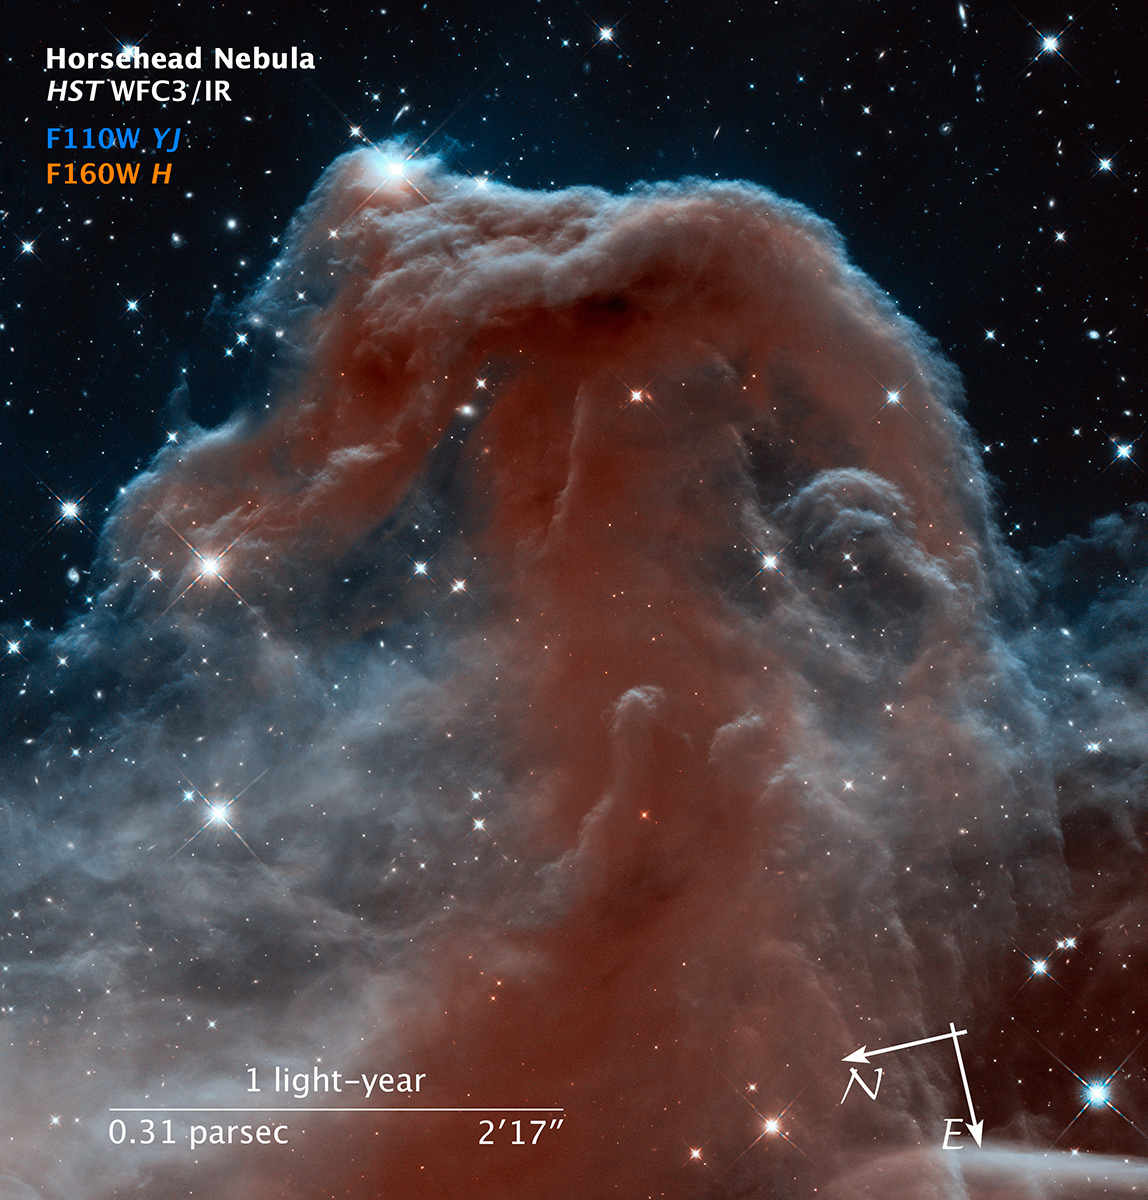
\includegraphics[width=.8\textwidth,keepaspectratio]{horsehead_hst.jpg}
%     % \caption{\href{https://hubblesite.org/contents/media/images/2013/12/3166-Image.html?keyword=Horsehead}{Horsehead Nebula captured by the Hubble Space Telescope (HST) in 2013.} The image was created from Hubble data from proposal \href{http://archive.stsci.edu/proposal_search.php?mission=hst&id=12812}{12812}. Illustration Credit: \href{http://www.nasa.gov/}{NASA}, \href{http://www.spacetelescope.org/}{ESA}, and Z. Levay (\href{http://www.stsci.edu/}{STScI})} 
% \end{figure}

% \begin{minipage}[t]{0.4\textwidth} 
% \begin{flushleft}
%     \large
%     \textbf{Student}\\
%     Ducheng Lu\\[1em]
% \end{flushleft}
% \end{minipage}
% \hfill 
% \begin{minipage}[t]{0.5\textwidth} 
%     \begin{flushright}
%         \large
%         \textbf{Supervisors}\\
%         Franck Le Petit (LERMA)\\
%         Emeric Bron (LERMA)
%         \vskip1em
%         Jan 2025
%     \end{flushright}
% \end{minipage}
% \vspace*{3em}

%%%%% cover page with background %%%%%
\newgeometry{top=.2in, bottom=0in, left=0in, right=0in} 
\thispagestyle{empty}
\large \hspace*{.2em} M2 International Research Track \hspace*{14em} Lab Insertion Unit Report\\[.2em]
\hspace*{-.24em}
\begin{overpic}[width=\paperwidth,height=.94\paperheight,keepaspectratio]{horsehead_hst.png}
    \put(2, 94){
\includegraphics[width=.7\textwidth,keepaspectratio]{Observatoire_de_Paris-CoMarquageLERMA-Blanc.png}}
    \put(0, 75){\textcolor{white}{\rule{\textwidth}{2pt}}} 
    \put(6, 69){\textcolor{white}{\huge Explaining Spectral Line Profiles in the Horsehead}} 
    \put(15, 65){\textcolor{white}{\huge Nebula Using Cloud Surface Curvature}} 
    \put(0, 60){\textcolor{white}{\rule{\textwidth}{2pt}}}

    \put(5, 25){\begin{minipage}[t]{0.3\textwidth} 
        \Large
        \textcolor{white}{
        Student\\
        Ducheng Lu}
    \end{minipage}}
    \put(35, 25){\begin{minipage}[t]{0.46\textwidth}
        \Large
        \begin{flushright}
            \textcolor{white}{
            Supervisors\\
            Franck Le Petit (LERMA)\\
            Emeric Bron (LERMA)\\
            \vskip1em
            Jan 2025}
        \end{flushright}
    \end{minipage}}
\end{overpic}
\restoregeometry
\normalsize

\clearpage
\thispagestyle{empty}
\begin{abstract}
\normalsize

The interstellar medium (ISM), composed of gas and dust between stars in galaxies, plays a critical role in star formation and galactic evolution. Interactions between the ISM and massive stars or star clusters shape its physical and chemical properties. One key region where these processes take place is the photodissociation region (PDR), where far-ultraviolet radiation dominates the chemical and heating processes. PDRs are the primary sources of infrared line and continuum radiation in galaxies, which are essential for probing PDR properties. PDR models have been instrumental in interpreting observational data; however, they have limitations, such as the use of one-dimensional slab geometry. This project develops a wrapper for the \mdpdr{} to compute column densities in spherical geometry and convolve them with instrument resolution, offering a more accurate model of line emission. These modifications improve the alignment between model and observed spatial profiles of emission lines along a cut in the Horsehead Nebula, both in shape and extent. Additionally, preliminary work on solving radiative transfer along the line of sight in spherical geometry is presented. The solution for radiative transfer in spherical geometry is still under development, and further improvements in profile modeling are anticipated. This work will enhance the interpretation of observational data and the determination of physical parameters from PDR models.

\end{abstract}

\begin{abstract}
\normalsize

Le milieu interstellaire (MIS), composé de gaz et de poussières entre les étoiles des galaxies, joue un rôle essentiel dans la formation des étoiles et l'évolution des galaxies. Les interactions entre le MIS et les étoiles massives ou les amas d'étoiles façonnent ses propriétés physiques et chimiques. Une région clé où ces processus ont lieu est la région de photodissociation (PDR), où le rayonnement ultraviolet lointain domine les processus chimiques et de chauffage. Les régions de photodissociation sont les principales sources de raies et de rayonnement continu dans le domaine infrarouge des galaxies, ce qui est essentiel pour sonder les propriétés des régions de photodissociation. Les modèles PDR ont joué un rôle important dans l'interprétation des données d'observation; cependant, ils ont des limites, comme l'utilisation d'une géométrie unidimensionnelle. Ce projet développe un wrapper pour le code \mintinline{python}{MeudonPDR} afin de calculer les densités de colonne en géométrie sphérique et de les convoluer avec la résolution de l'instrument, offrant un modèle plus précis des profils spatiaux d'émission des raies. Ces modifications améliorent l'alignement entre le modèle et les profils spatiaux de raies le long d'une coupe dans la nébuleuse de la Tête de Cheval, à la fois en termes de forme et d'étendue. En outre, des travaux préliminaires sur la résolution du transfert radiatif le long de la ligne de visée en géométrie sphérique sont présentés. La solution pour le transfert radiatif en géométrie sphérique est encore en cours de développement, et d'autres améliorations dans la modélisation des profils sont attendues. Ce travail améliorera l'interprétation des données d'observation et la détermination des paramètres physiques à partir des modèles PDR.

\end{abstract}

\clearpage
\thispagestyle{empty}
\vspace*{\fill}
{\hypersetup{hidelinks}\large
\tableofcontents
}
\vspace*{\fill}

\begingroup
\renewcommand{\thefootnote}{}
\footnotetext{cover page image: \href{https://hubblesite.org/contents/media/images/2013/12/3166-Image.html?keyword=Horsehead}{Horsehead Nebula captured by the Hubble Space Telescope (HST) in 2013.} The image was created from Hubble data from proposal \href{http://archive.stsci.edu/proposal_search.php?mission=hst&id=12812}{12812}. Illustration Credit: \href{http://www.nasa.gov/}{NASA}, \href{http://www.spacetelescope.org/}{ESA}, and Z. Levay (\href{http://www.stsci.edu/}{STScI})}
\endgroup

\clearpage
\pagenumbering{arabic}
\section{Introduction}

The interstellar medium (ISM), composed of gas and dust between stars in galaxies, plays a critical role in star formation and galactic evolution, constituting approximately $10\%$ of the total baryonic mass \parencite{Draine2011}. The ISM is a dynamic environment where radiation, cosmic rays, magnectic fields, and turbulence interact with gas and dust, shaping its physical and chemical properties. It is the main site of star formation and serves as a matter reservoir for this process. In turn, massive stars and star clusters can disturb nearby molecular clouds through their strong stellar winds, ultraviolet (UV) radiation, and, at times, transient events like supernovae. This influence extends across various regions, from the diffuse edges of molecular clouds to their cold, dense cores. One such key region where these processes take place is the photodissociation region (PDR), which forms at the interface between molecular clouds and sources of UV radiation. 

\subsection{Photodissociation Regions (PDRs)}
Photodissociation regions (PDRs) are regions of neutral gas in the ISM where far-ultraviolet (FUV; $\qty{6}{eV} < h\nu < \qty{13.6}{eV}$) radiation dominates the chemical and heating processes \parencite{Tielens1985}. A PDR begins at the ionization front (IF), where photons with energies above the Lyman limit (\qty{13.6}{eV}) are fully absorbed, preventing further ionization of hydrogen. PDRs span a wide range of incident FUV fluxes and densities, including all neutral gas in the ISM and molecular layers where FUV radiation drives molecule formation.

\begin{figure}[hb]
    \centering
    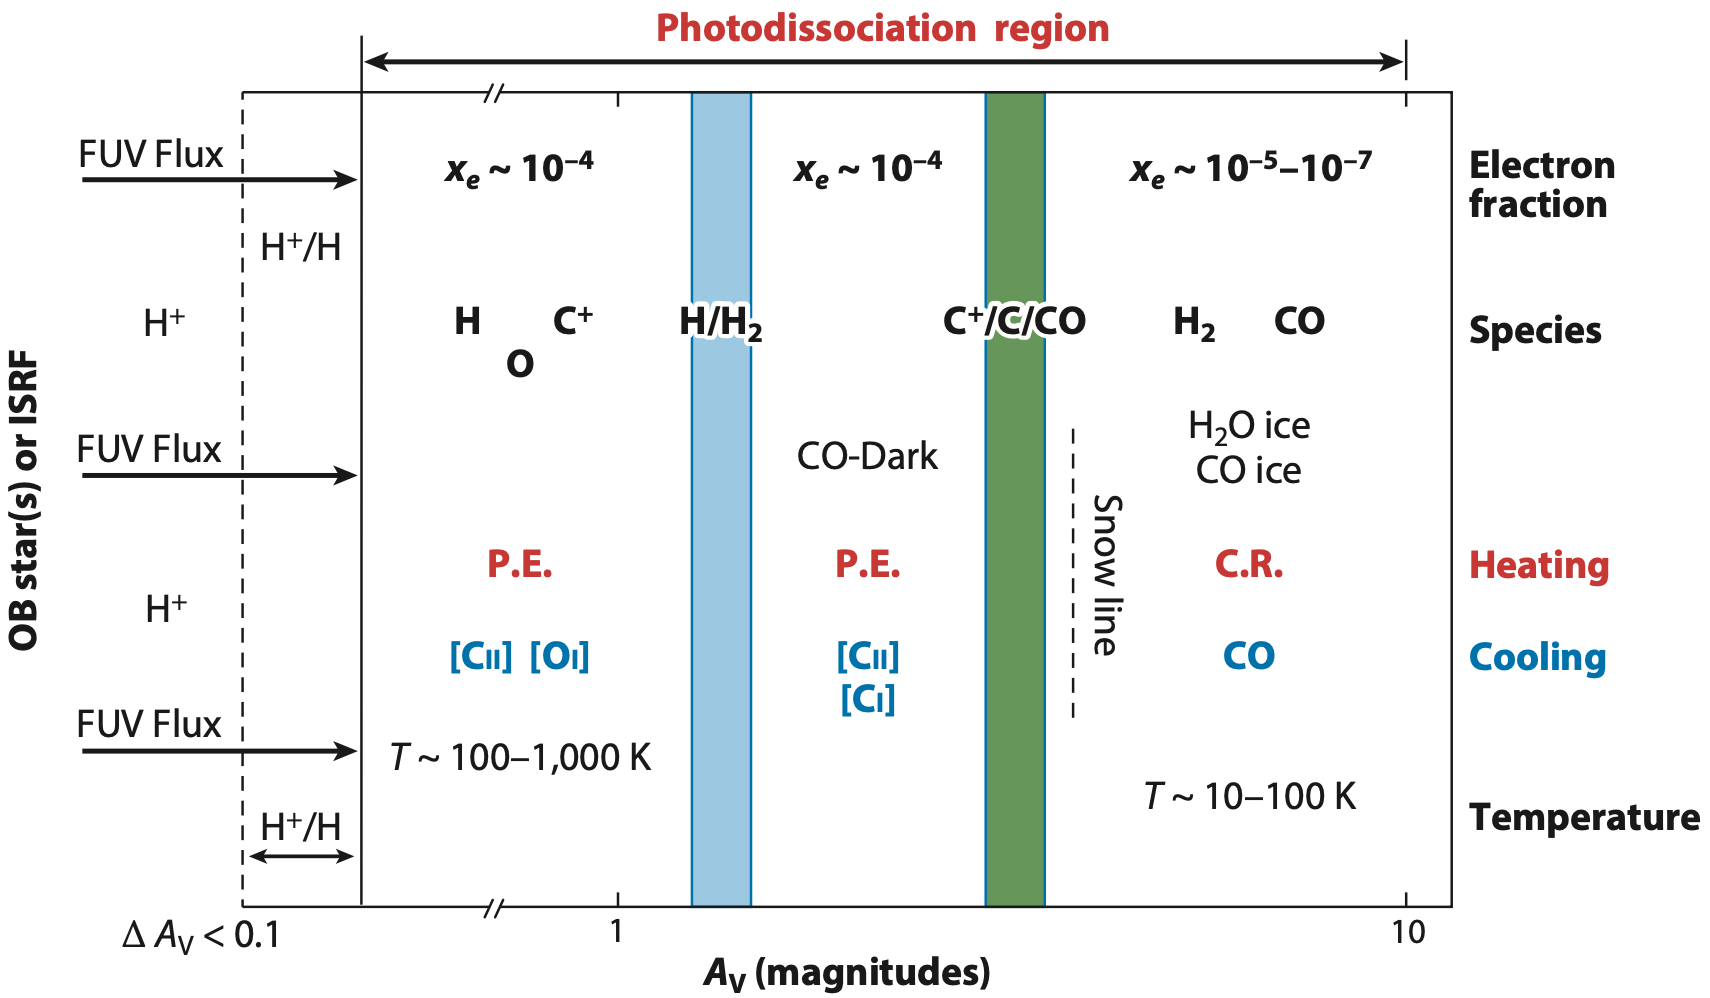
\includegraphics[width=.7\textwidth,keepaspectratio]{figures/PDRScheme.png}
    \caption{Schematic of a photodissociation region as a function of visual extinction $A_V$. Reprinted from \textcite{Wolfire2022}, Fig.~2. Red text indicates the dominant heating mechanisms, with "P.E." referring to photoelectric effects and "C.R." referring to cosmic rays. Blue text represents the main line emissions, which are the main cooling mechanisms.} \label{fig:pdrscheme}
\end{figure}

PDRs are the primary sources of infrared (IR) line and continuum radiation in galaxies \parencite{Crawford1985,Stacey2010}. Grains absorb the majority of the FUV radiation and re-radiate it in the IR continuum, but a fraction of the FUV photons heat the gas through photoelectric effect, which then cool through line emission. Together, the line and continuum emission provide important insights into the physical and chemical conditions in PDRs. The study of PDRs is vital for understanding star formation and galaxy evolution. Observations of PDRs help to constrain key physical parameters such as temperature, chemical composition, and radiative energy, probing the local environments of star-forming regions and the potential presence of stellar feedback.

Fig.~\ref{fig:pdrscheme} shows a one-dimensional (1D) structure of PDR illuminated by radiation field from the left. The adjacent \ce{H_{II}} region absorbs extreme-ultraviolet (EUV; $h\nu > \qty{13.6}{eV}$) photons, leaving FUV photons that create the PDR. Atomic hydrogen, helium, and oxygen are neutral because their ionization potentials exceed \qty{13.6}{eV}, while molecules are photodissociated, and metals like carbon, silicon, and sulfur are singly ionized. The heating process is dominated by photoelectric effect on small grains and polycyclic aromatic hydrocarbons (PAHs), and the cooling process is dominated by fine-structure line emission. As the depth increases and FUV radiation diminishes, \ce{H2} forms, followed by \ce{CO}. Both \ce{H2} and \ce{CO} photodissociate via line absorption and can therefore self-shield, allowing them to form closer to the surface than other molecules like \ce{H2O} and its isotopologues, which dissociate via FUV continuum. In the deepest layers, cosmic rays dominate the heating process, and rotational transitions of \ce{CO} isotopologues become the primary coolants.

\subsection{The Horsehead Nebula}
% \begin{figure}
%     \centering
%     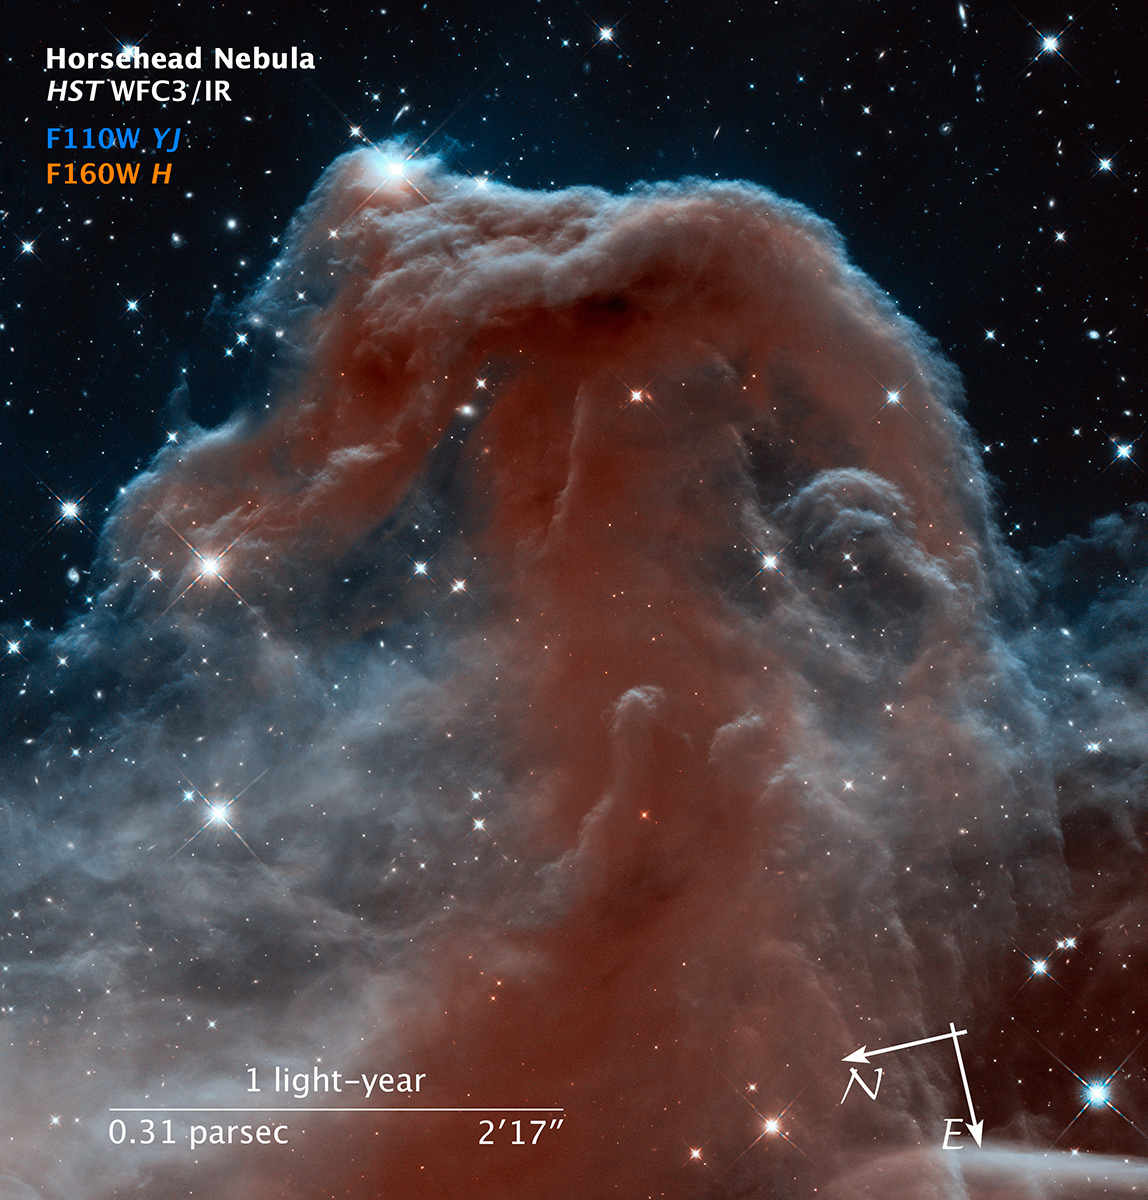
\includegraphics[width=.7\textwidth,keepaspectratio]{horsehead_hst.jpg}
%     \caption{\href{https://hubblesite.org/contents/media/images/2013/12/3166-Image.html?keyword=Horsehead}{Horsehead Nebula captured by the Hubble Space Telescope (HST) in 2013.} The image was created from Hubble data from proposal \href{http://archive.stsci.edu/proposal_search.php?mission=hst&id=12812}{12812}. Illustration Credit: \href{http://www.nasa.gov/}{NASA}, \href{http://www.spacetelescope.org/}{ESA}, and Z. Levay (\href{http://www.stsci.edu/}{STScI})} 
% \end{figure}

% \begin{figure}
%     \centering
%     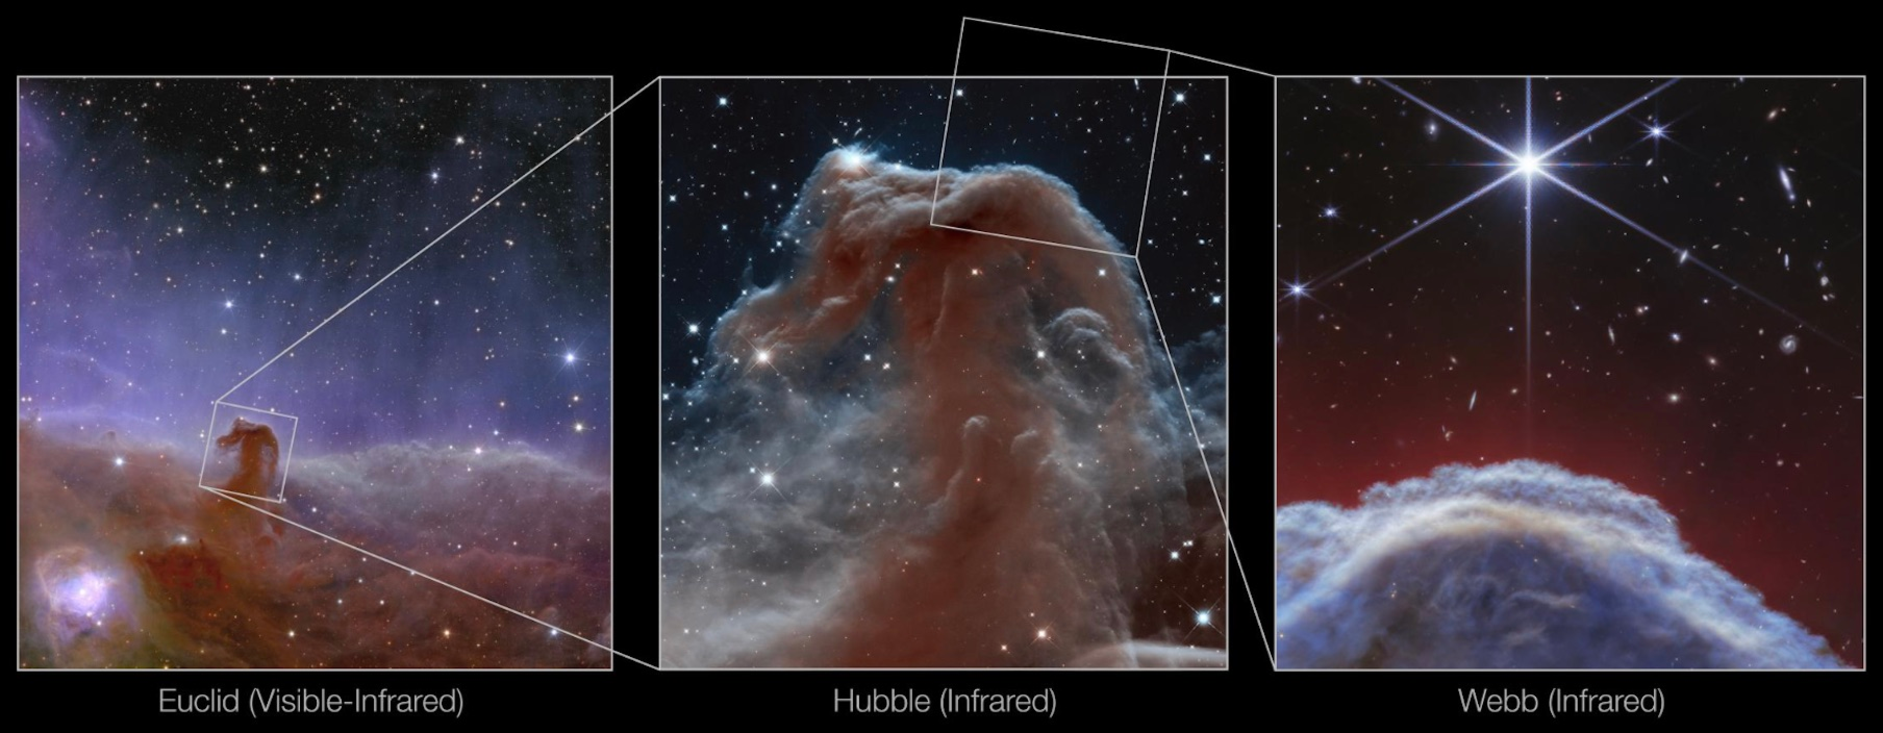
\includegraphics[width=\textwidth,keepaspectratio]{horsehead_zoomed.pdf}
%     \caption{\href{https://www.esa.int/ESA_Multimedia/Images/2024/04/Webb_captures_iconic_Horsehead_Nebula_in_unprecedented_detail}{Three views of the Horsehead Nebula}. The first image (left) features the Horsehead Nebula as seen by ESA's Euclid telescope. The second image (middle) shows the NASA/ESA Hubble Space Telescope's infrared view of the Horsehead Nebula. The third image (right) features a new view of the Horsehead Nebula from the NASA/ESA/CSA James Webb Space Telescope's NIRCam (Near-InfraRed Camera) instrument.}
% \end{figure}

The Horsehead Nebula (Fig.~\ref{fig:obsimg} and cover image) is a well-known PDR that has been extensively studied in the literature. It is illuminated by $\sigma$ Orionis, a O9.5V binary star system \parencite{Warren1977}, located 3.5 pc from the edge of the PDR \parencite{Abergel2003,Schirmer2020}, resulting in an incident FUV radiation field of around \qty{2.7e-3}{erg\,\second^{-1}\,\centi\metre^{-2}} \parencite{Habart2005}. 

\begin{figure}[ht]
    \centering
    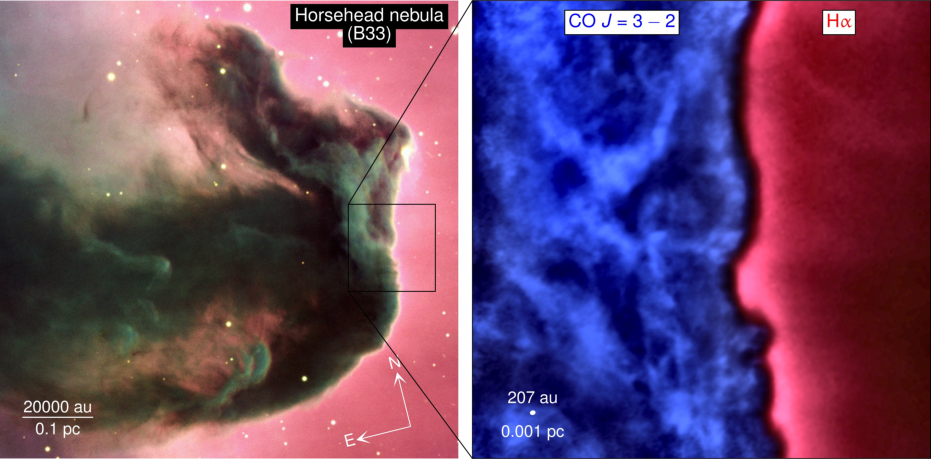
\includegraphics[width=\textwidth,keepaspectratio]{horsehead_HernandezVera2023.pdf}
    \caption{Multiphase view of the Horsehead nebula (Barnard 33). Reprinted from \textcite{HernándezVera2023}. Left: Composite color image of the Horsehead nebula observed with the VLT (ESO). Right: Zoomed-in view of the edge of the molecular cloud, imaged with ALMA in the \ce{CO} $J = 3-2$ line emission (blue) and the \qty{0.9}{m} KPNO telescope in the H$\alpha$ line emission. The dark region represents the neutral atomic layer.} \label{fig:obsimg}
\end{figure}

In observational studies, it is customary to use arcseconds as the distance unit. As the Horsehead PDR is located approximately \qty{400}{pc} from us \parencite{Menten2007, Schlafly2014}, the distance unit can be converted as:
\begin{equation}
    \alpha[''] = \frac{d\,[\unit{pc}]}{400\,\unit{pc}} \frac{1''}{1\,\unit{rad}}.
\end{equation}
This gives \(1''\) corresponding to \qty{1.9}{mpc}. The horsehead PDR is nearly edge-on, with an upper limit for the angle of $6^\circ$ \parencite{Habart2005}.

% For lines that are optically thin, the local emissitivity is given by
% \begin{equation}
%     \epsilon_{ul} \simeq \frac{1}{4\pi}A_{ul}n_u h\nu_{ul} \propto n_u
% \end{equation}

\subsection{Motivation}
% While 1D PDR models have been instrumental in advancing our understanding of PDRs, they come with some limitations. Classic PDR models assume a 1D slab geometry, treating the cloud structure as uniform along a single line of sight (LoS). This simplification has proven quite helpful, as it allows for detailed simulations of other physical and chemical processes. However, in reality, the curvature of the PDR surface introduces variations in physical conditions within the same telescope beam. Accounting for this curvature is crucial to accurately reproduce the observed line profiles. 

% Another limitation of classic PDR models is their omission of absorption of line emission by the cloud itself. As emission lines propagate in PDRs, they can be absorbed along the LoS and become optically thick, potentially leading to inaccurate line ratios and distorted profiles \parencite{Abel2007,Guevara2020}.

% These limitations can hinder the accurate interpretation of observational data and the determination of physical parameters derived from PDR models. As a result, there is a growing demand for more advanced models that deal with the curvature of PDR surfaces. To address these challenges, this project aims to develop a wrapper for the \mdpdr{}. The wrapper will extend the output of the 1D model by computing column densities in spherical geometry. Additionally, the project will explore solving the radiative transfer equation along the line of sight (LoS), providing a more accurate representation of PDR line emission and its propagation through the medium. This project is part of a collaboration between JPL (Darek Lis), Paris Observatory (us), IRAM (David Teyssier), and CSIC Madrid (Javier Goicoechea) to study the presence of water in the Horsehead Nebula. More generally, we aim to explain the localization of several emission lines, including \ce{H2O}, \ce{C}, \ce{^{12}CO}, \ce{^{13}CO}, and \ce{^{18}CO} in the Horsehead.

While 1D PDR models have been instrumental in advancing our understanding of PDRs, they come with some limitations. Classic PDR models assume a 1D slab, plane-parallel geometry, which treats the cloud as infinite and uniform in two directions and describes its state only as a function of depth along the direction of the surface normal. In reality, PDRs have complex, wavy and corrugated surfaces. Due to limb brightening, the parts of the surface observed edge-on appear brighter. These edge-on observations are important because they provide direct observational access to the chemical stratification of the PDR, and hence, the stratification of the emission of different species. However, the curvature of the surface affects the observed spatial emission profiles, as the line of sight (LoS) passes through gas at different depths from the surface. This can distort the observed line profiles, hindering the accurate interpretation of observational data and the determination of physical parameters derived from PDR models. As observations of edge-on PDRs become more capable of resolving the stratification of emission, there is a growing demand for more advanced models that can directly compare the predicted spatial structure with such observations, instead of predictions based on infinite slab geometries.

One potential solution is to approximate the surface near the edge-on regions by its curvature radius. The simplest starting point for this approach is to map the 1D model to spherical geometry. Building on this concept, this project aims to develop a wrapper for \mdpdr{} that will compute observable spatial profiles of column densities on a spherical PDR surface and, preliminarily, line intensities by solving the radiative transfer along each LoS. To test the effectiveness of this method, the Horsehead Nebula serves as an ideal case study, as it is an edge-on PDR with available spatial emission data from several tracers.

This project is part of a collaboration between JPL (Darek Lis), Paris Observatory (us), IRAM (David Teyssier), and CSIC Madrid (Javier Goicoechea) to study the presence of water in the Horsehead Nebula. More generally, we aim to explain the localization of several emission lines, including \ce{H2O}, \ce{C}, \ce{^{12}CO}, \ce{^{13}CO}, and \ce{^{18}CO} in the Horsehead.

The report is organized as follows: Sec.~\ref{sec:data} describes the observational data used in this study. Sec.~\ref{sec:methods} outlines the methods. Specifically, in Sec.~\ref{sec:mdpdr}, I provide an overview of the \mintinline{python}{MeudonPDR} models, with Secs.~\ref{sec:cstnp}, \ref{sec:exactrt}, and \ref{sec:surfchem} describing how model parameters are determined, including comparisons between constant density and constant pressure models, the effects of the exact method of radiative transfer, and the effects of surface chemistry, respectively. In Sec.~\ref{sec:sphere}, I describe how column densities are computed for a spherical PDR surface. Sec.~\ref{sec:rte} discusses the solution of the radiative transfer equation along the LoS. Sec.~\ref{sec:convolution} outlines the process of convolving model outputs with instrumental resolution. Sec.~\ref{sec:results} presents the results, with Sec.~\ref{sec:convcolden} focusing on the convolved column densities, Sec.~\ref{sec:comprad} on the effects of varying cloud radius, and Sec.~\ref{sec:comprte} on the preliminary results of considering radiative transfer. Finally, Sec.~\ref{sec:conclusion} summarizes the conclusions and discusses the prospects of the study.

\section{Data} \label{sec:data}
The observational data used in this study (Fig.~\ref{fig:observation}) were obtained from two instruments: the Heterodyne Instrument for the Far-Infrared (HIFI) \parencite{deGraauw2010} onboard the Herschel Space Observatory \parencite{Pilbratt2010}, and the IRAM-30m telescope \parencite{Baars1987}. These data were taken along a cut through the Horsehead Nebula and were provided by Darek Lis. For consistency, all spatial profiles were convolved to a common spatial resolution of $38.1$ arcsec, the resolution of the HIFI \ce{H2O} observation, which has the lowest resolution among the observed lines.  The molecular species observed, including \ce{H2O}, \ce{C}, \ce{^{12}CO}, and \ce{^{18}CO}, were detected at specific wavelengths corresponding to the transitions listed in Table.~\ref{tab:lines}.

\begin{figure}[h!]
    \centering
    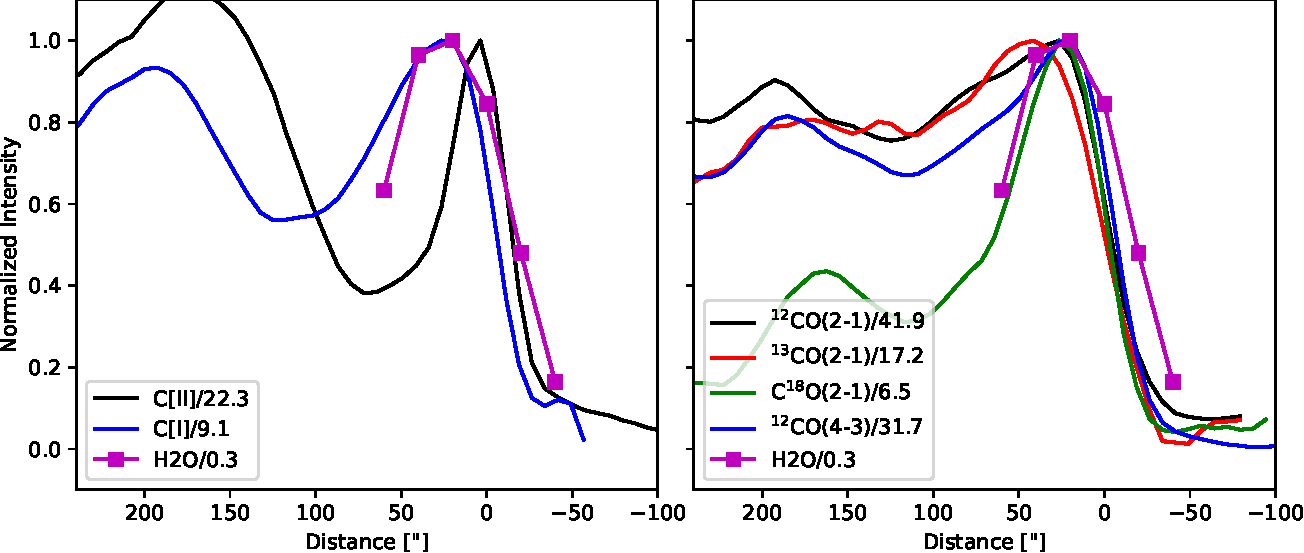
\includegraphics[width=\textwidth,keepaspectratio]{observed_lines.pdf}
    % \caption{Observed line profiles of the Horsehead Nebula obtained with Herschel HIFI. Data provided by Darek Lis.  Due to bad weather conditions during the observation of the \ce{^{13}CO} line, it will not be considered in later comparisons.} \label{fig:observation}
    \caption{Observed line profiles of the Horsehead Nebula obtained with Herschel HIFI. Data provided by Darek Lis.} \label{fig:observation}
\end{figure}

\begin{table}[h!]
    \centering
    \begin{tabular}{cclll}
        \midrule
        \midrule
        Notation & Species & Upper Level & Lower Level & Frequency (\unit{GHz}) \\
        \midrule
        \ce{H2O}            & \ce{H2O}  & J=1, Ka=1, Kc=0 & J=1, Ka=0, Kc=1 & 557.30 \\
        \ce{C[II]}          & \ce{C+}   & 2P J=3/2 & 2P J=1/2 & 1902.59 \\
        \ce{C[I]}           & \ce{C}    & 3P J=1 & 3P J=0 & 492.02 \\
        \ce{CO} (2-1)       & \ce{CO}   & v=0, J=2 & v=0, J=1 & 230.538 \\
        \ce{CO} (4-3)       & \ce{CO}   & v=0, J=4 & v=0, J=3 & 461.041 \\
        % \ce{^{13}CO} (2-1)  & \ce{^{13}CO} & v=0, J=2 & v=0, J=1 & 220.399 \\
        \ce{C^{18}O} (2-1)  & \ce{C^{18}O} & v=0, J=2 & v=0, J=1 & 219.560 \\
        \midrule
        \bottomrule
    \end{tabular}
    \caption{Parameters of transitions in the observation data used in this study.} \label{tab:lines}
\end{table}

\section{Methods} \label{sec:methods}
\subsection{The \mdpdr{}} \label{sec:mdpdr}
A significant heterogeneity exists among the available PDR models, which differ in their geometry, physical and chemical structures, and model parameters. \textcite{Röllig2007} suggest that the choice of a spedific code should depend on the physical and chemical processes implemented in the code, as well as the characteristics of the emission source. 

In this project, I used the \mdpdr{} \parencite{LePetit2006,Goicoechea2007,Gonzalez2008,LeBourlot2012,Bron_thesis,Bron2014,Bron2016} to simulate the Horsehead Nebula. The \mdpdr{} models a stationary, 1D slab of gas and dust illuminated by a UV radiation field from one or both sides (Fig.~\ref{fig:1Dgeometry}). At each iteration, the code self-consistently solves the radiative transfer in both lines and continuum (from the UV to the radio domain), the chemical balance, the statistical equilibrium for level populations, and the thermal balance, all of which are deeply coupled to one another. The code outputs the level populations, gas temperature, and chemical abundances as a function of depth into the cloud, with optional output of the radiation field. The physical parameters used to model the Horsehead PDR are summarized in Table.~\ref{tab:params}.

\begin{table}[h!]
    \centering
    \begin{tabular}{ll}
        \midrule
        \midrule
        Cloud size ($A_{V, \max}$\footnotemark[1]) & 40 \\
        Proton density\footnotemark[2] ($n_H$) & \qtyrange[range-units=single,range-phrase=~--~]{3e4}{3e6}{cm^{-3}}\\
        Pressure\footnotemark[2] ($P$) & \qtyrange[range-units=single,range-phrase=~--~]{1e6}{1e7}{K\,cm^{-3}} \\
        ISRF & shape: Mathis\footnotemark[3], geometry: beam\_isot\footnotemark[4] \\
        ISRF scaling factor & $G_0^\mr{obs} = 100,\ G_0^\mr{back} = 0.04$\footnotemark[5]\\
        UV radiative transfer method & FGK approximation, or\\
        & exact \ce{H2} self- and mutual shielding\footnotemark[6] \\
        Turbulent velocity dispersion & \qty{2}{\km\per\second}\footnotemark[7] \\
        Extinction Curve & HD38087\footnotemark[8]\\
        $R_V = A_V / E(B-V)$\footnotemark[9] & $5.50$ \\
        $C_D = N_H / E(B-V)$\footnotemark[9] & $1.57\times 10^{22}$\\
        \bottomrule
    \end{tabular}
    \caption{Key physical parameters used to model the Horsehead PDR in the \mdpdr{}.\textsuperscript{(1)}Total visual extinction of the slab, \(A_V \equiv 2.5\log_{10}(I_\mr{V}^0/I_\mr{V}^\mr{obs})\). \textsuperscript{(2)}Proton density is used in constant density models, and pressure is used in constant pressure models (see Sec.~\ref{sec:cstnp}). \textsuperscript{(3)}Radiation field shape from \textcite{Mathis1983}. \textsuperscript{(4)}ISRF geometry: beam perpendicular on the observer side, isotropic on the back side. \textsuperscript{(5)}ISRF scaling factors are in Habing units, as defined in \textcite{LePetit2006}. \textsuperscript{(6)}UV radiative transfer methods include the FGK approximation or exact \ce{H2} shielding (see Sec.~\ref{sec:exactrt}). \textsuperscript{(7)}Turbulent velocity dispersion is used only for Doppler line broadening. \textsuperscript{(8)}Extinction curve from \textcite{Fitzpatrick1990}. \textsuperscript{(9)}Parameters related to extinction. Other parameters use default values. More descriptions can be found in the \href{https://ism.obspm.fr/files/PDRDocumentation/PDRDoc7.pdf}{\mintinline{latex}{MeudonPDR}} documentation.} \label{tab:params}
\end{table}

\begin{figure}
    \centering
    % \includegraphics[width=.6\textwidth,keepaspectratio]{slab_geometry.png}
    % \caption{Scheme of the slab geometry of the \mdpdr{}. Reprinted from \textcite{LePetit2006}.} \label{fig:1Dgeometry}
    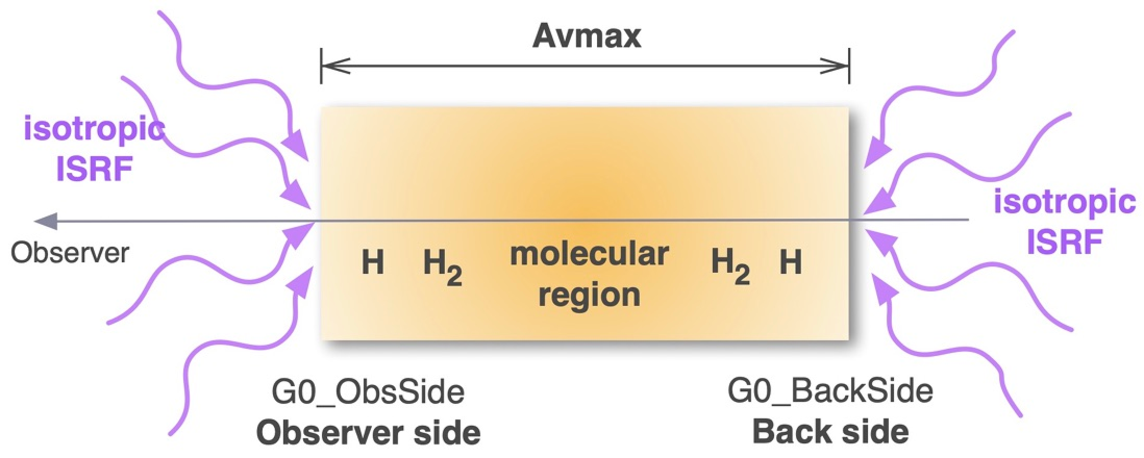
\includegraphics[width=.7\textwidth,keepaspectratio]{schemePDR.pdf}
    \caption{Scheme of the slab geometry in \mdpdr{}. $A_V = 0$ at the observer side and increases toward the back side, reaching $A_V = A_{V, \max}$, which controls the size of the cloud. Reprinted from Fig.~3.1 in \href{https://ism.obspm.fr/files/PDRDocumentation/PDRDoc7.pdf}{\mintinline{latex}{MeudonPDR}} documentation.} \label{fig:1Dgeometry}
\end{figure}

In a complex model such as the \mdpdr{}, different levels or types of approximations are possible. It is therefore necessary to decide what is adequate for this study. In the following sections, I investigate the impact of three of the most important choices on the PDR structure. First, since the code does not solve the hydrodynamics of the gas, either a constant pressure or a constant density profile must be assumed. Second, the modeling of \ce{H2} self-shielding and the shielding of \ce{CO} by \ce{H2} is examined. The FGK approximation, which treats each line independently in the UV transfer and neglects overlaps between absorption lines of \ce{H2} or between lines of \ce{H2} and other species such as \ce{CO}, is compared to the “exact” transfer approach, which fully accounts for these overlaps. Finally, the inclusion of surface chemistry is considered. By default, the \mdpdr{} includes surface chemistry only for \ce{H2} formation, as surface processes often have little impact on some other PDR tracers. However, whether surface chemistry is significant for this study remains to be verified.

\subsubsection{Constant Pressure vs. Constant Density} \label{sec:cstnp}

The density structure of a PDR model, whether it assumes constant density, constant pressure, or a user-defined density profile, can significantly influence the simulation results \parencite{Wolfire2022}. As shown in Fig.~\ref{fig:cmp_cstp_cstn} and Fig.~\ref{fig:cmp_cstp_cstn_arcsec}, I compare the cloud structure computed with constant pressure and constant density assumptions, illustrating the differences in the resulting PDR structures. The values $n_H = \qty{3e5}{cm^{-3}}$ for the constant density model and $P = \qty{5e6}{K\,cm^{-3}}$ for the constant pressure model are based on \textcite{Maillard2023}. 

% In the constant pressure model, the transition from atomic to molecular hydrogen occurs at higher visual extinction (Fig.~\ref{fig:cmp_cstp_cstn}), and the total physical thickness of the cloud is larger (Fig.~\ref{fig:cmp_cstp_cstn_arcsec}). The temperature profile in the constant pressure model is also more gradual. Additional comparisons between various constant density models and constant pressure models are provided \qt{in the appendix}.

% - the spatial structure in function of Av are qualitatively similar (except for what happens with carbon and water near the H/H2 transition)
% - what happens near the H/H2 transition in the constant density model, is a result of having a much higher density for this region than the constant pressure model. 
% - The temperature in the atomic region is also much higher in the atomic region for the constant density model, also because of the higher density.
% - in physical distance, the constant pressure model has a much more extended atomic region (because high temperature, so low density) and a much more compressed molecular region (because low temperature, so high density). 

The PDR structure as a function of $A_V$ in the constant density and constant pressure models differs most in the behavior of carbon and water near the \ce{H/H2} transition (Fig.~\ref{fig:cmp_cstp_cstn}), due to the much higher density in the constant density model. Additionally, the temperature in the atomic region is higher in the constant density model than in the constant pressure model. This occurs because, in the constant density model, the surface layer is much denser and absorbs UV radiation more efficiently. In contrast, in the constant pressure model (fixed $P = nkT$), the density increases gradually from the surface to deeper regions as the temperature decreases. Consequently, in physical distance (Fig.~\ref{fig:cmp_cstp_cstn_arcsec}), the constant pressure model has a more extended atomic region and a more compressed molecular region. Additional comparisons between various constant density models and constant pressure models are provided in the appendix.

Observations of the Horsehead Nebula reveal a steep density gradient in the PDR \parencite{Habart2005,Guzmán2011}. \textcite{HernándezVera2023} showed that constant density models fail to reproduce the observed structures, and neither do previously proposed density profile prescriptions. Furthermore, recent observations from ALMA and Herschel indicate that the warm layer of PDRs is indeed isobaric, with relatively high thermal pressures \parencite{Marconi1998,Goicoechea2016,Joblin2018,Wu2018,Bron2018,Maillard2021}. Based on these findings, I adopt a constant pressure model with $P = \qty{5e6}{K\,cm^{-3}}$ for the subsequent analysis.

\begin{figure}[ht]
    \centering
    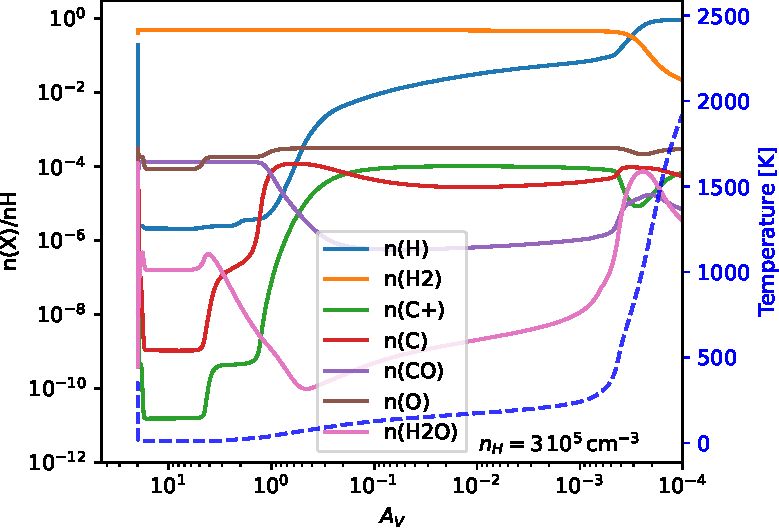
\includegraphics[width=.49\textwidth,keepaspectratio]{struct_nH3e5.pdf}
    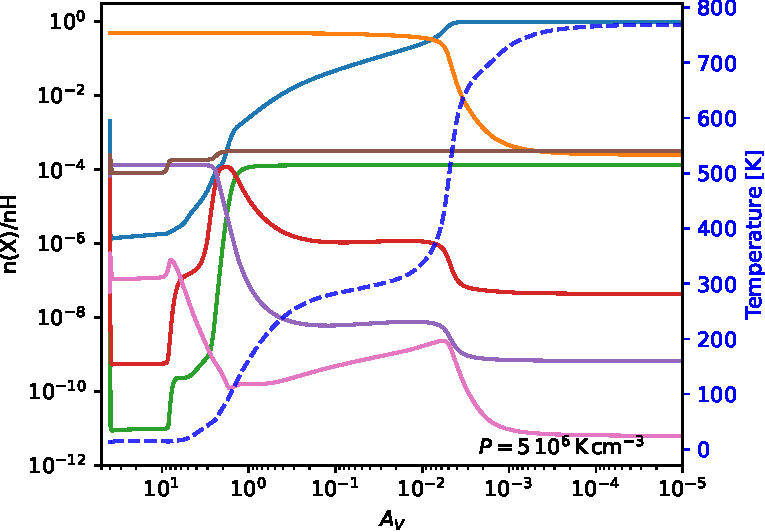
\includegraphics[width=.49\textwidth,keepaspectratio]{struct_P5e6.pdf}
    \caption{Comparison of the cloud structure computed with constant density $n_H = \qty{3e5}{cm^{-3}}$ (left) and constant pressure $P = \qty{5e6}{K\,cm^{-3}}$ (right), with a shared legend displayed in the left plot. The blues represent temperature and correspond to the right axes. All other parameters are the same as those listed in Table.~\ref{tab:params}. Note that the radiation field is now coming from the right to conform with the observation, so $A_V$ increases from right to left.} \label{fig:cmp_cstp_cstn}
\end{figure}

\begin{figure}[ht]
    \centering
    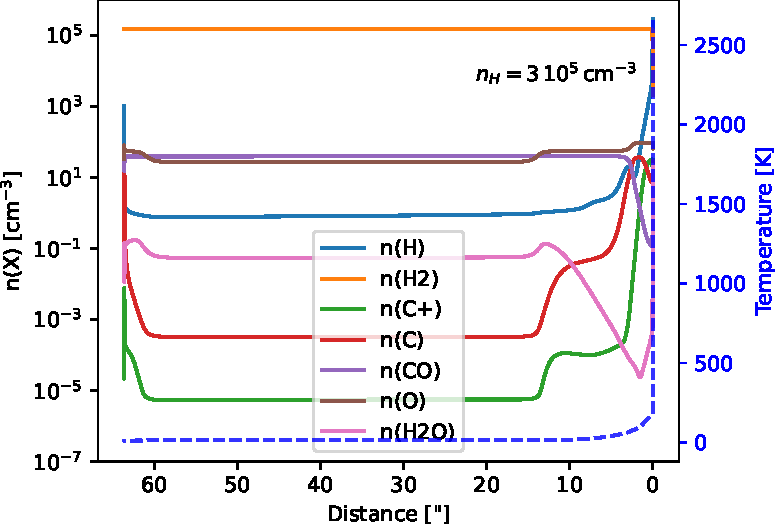
\includegraphics[width=.49\textwidth,keepaspectratio]{struct_nH3e5_arcsec.pdf}
    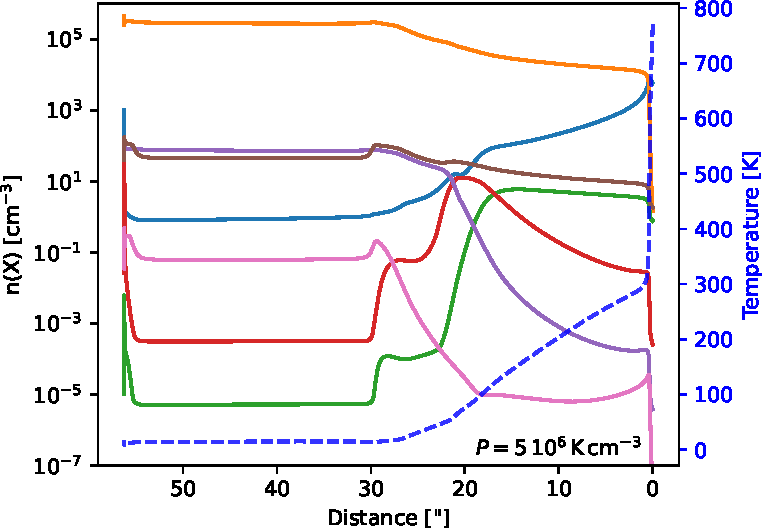
\includegraphics[width=.49\textwidth,keepaspectratio]{struct_P5e6_arcsec.pdf}
    \caption{Similar to Fig.~\ref{fig:cmp_cstp_cstn}, but using physical units, with arcseconds as the distance unit and the densities represented by their actual values (not normalized by proton density).} \label{fig:cmp_cstp_cstn_arcsec}
\end{figure}

\subsubsection{Models with Exact Radiative Transfer of \texorpdfstring{\ce{H2}}{H2}} \label{sec:exactrt}

There are two options available in the \mdpdr{} for treating radiative transfer in the UV. The first is the FGK approximation \parencite{Federman1979}, in which the self-shielding of \ce{H} and \ce{H2} molecules is treated approximately. Self-shielding occurs when molecules absorb radiation in their own spectral lines, reducing the flux available to penetrate deeper into the cloud. However, the FGK approximation neglects mutual shielding, where the overlap and interaction of absorption lines between different species or multiple lines of the same species further attenuate the radiation field.

\begin{figure}[h]
    \centering
    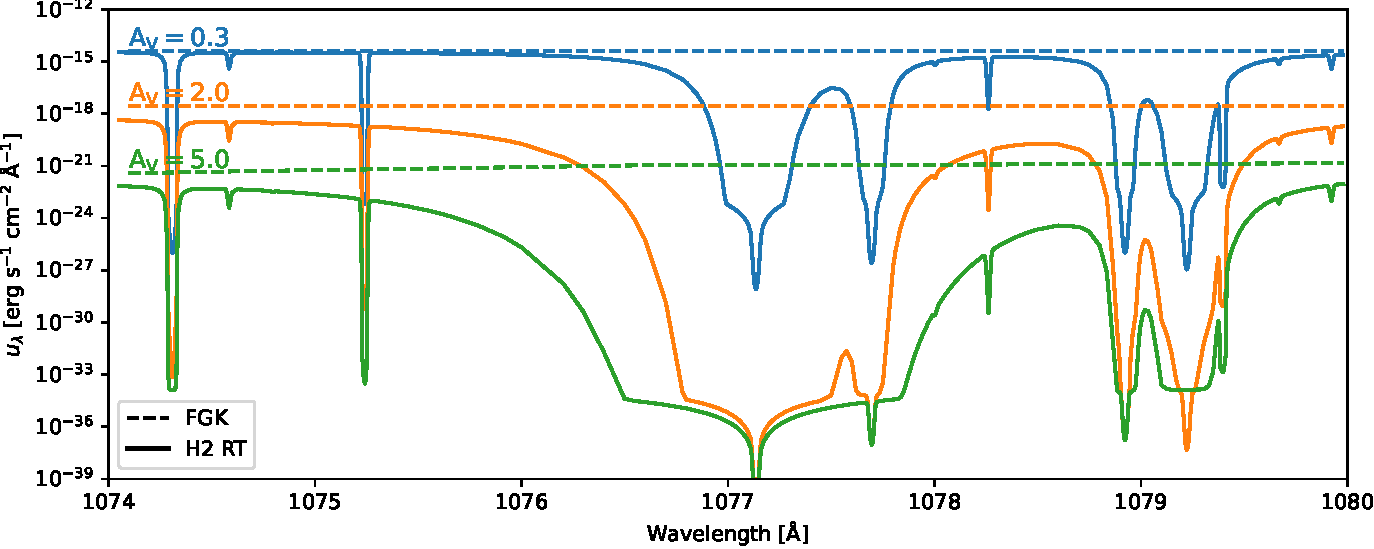
\includegraphics[width=.92\textwidth,keepaspectratio]{spectra_fgkh2_1.pdf}
    % 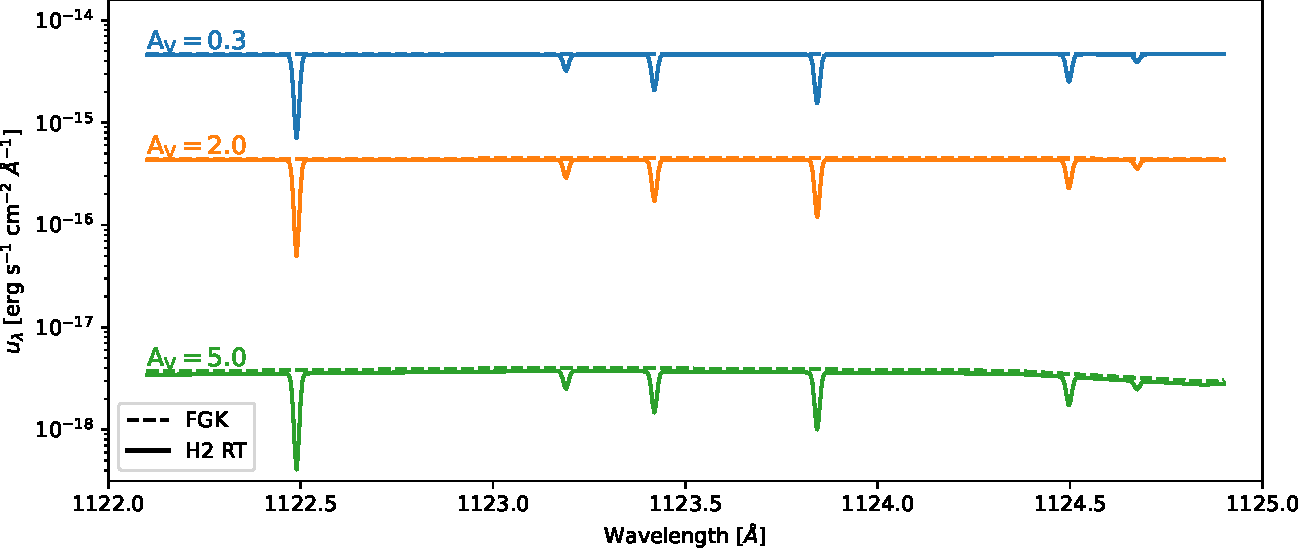
\includegraphics[width=.88\textwidth,keepaspectratio]{spectra_fgkh2_2.pdf}
    \caption{Comparison of the local energy density of the radiation field from $1074~\text{\AA}$ to $1080~\text{\AA}$ at visual extinction depths $A_V = 0.3$ (blue), $A_V = 2$ (orange), and $A_V = 5$ (green), for models computed using the FGK approximation (dashed lines) and the exact radiative transfer method (solid lines) including the 20 lowest \ce{H2} absorption lines. \qt{change the plot?}} \label{fig:cmpH2rtspectra}
\end{figure}

The second, more accurate approach is to solve the radiative transfer exactly, i.e., on a wavelength grid fine enough to resolve the multiple UV absorption lines of important species such as \ce{H}, \ce{H2}, and \ce{CO}. This method explicitly includes mutual shielding for absorption lines corresponding to a given number of energy levels of \ce{H}, \ce{H2}, \ce{D}, \ce{HD}, \ce{CO}, \ce{^{13}CO}, and \ce{C^{18}O}, as detailed in \textcite{Goicoechea2007, Gonzalez2008}. For higher energy levels, the FGK approximation is retained, as their contributions are negligible due to their low populations.

Fig.~\ref{fig:cmpH2rtspectra} compares spectra from $1074~\text{\AA}$ to $1080~\text{\AA}$ at various visual extinction values for models computed using the FGK approximation and the exact radiative transfer method, demonstrating pronounced attenuation when the exact radiative transfer of \ce{H2} in included. In the spectrum computed using the FGK approximation, the \ce{H2} lines appear absent in the FGK approximation because they are treated independently of the wavelength-dependent spectrum. However, Fig.~\ref{fig:cmpH2rtspectra} clearly shows that some \ce{H2} lines strongly overlap, an effect that eludes the FGK approximation.

This highlights the advantage of the exact radiative transfer method, which, although computationally more intensive, provides a more detailed treatment of the UV radiation field, thereby influencing the PDR structure. For instance, the exact method leads to increased attenuation of the radiation field, shifting the \ce{H}/\ce{H2} transition layer to lower extinction depths \parencite{Goicoechea2007}, as illustrated in Fig.~\ref{fig:cmpH2rt}. Furthermore, the enhanced attenuation from mutual shielding results in a lower temperature profile. To balance accuracy and computational efficiency, my model applies exact radiative transfer only to the 20 lowest energy levels of \ce{H2}, which are the primary contributors to the attenuation. 

\begin{figure}[ht]
    \centering
    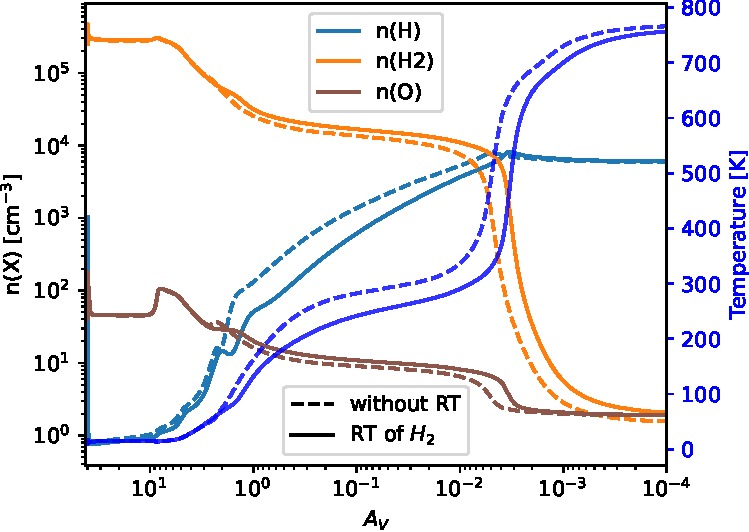
\includegraphics[width=.51\textwidth,keepaspectratio]{cmpH2rt_H_O.pdf}
    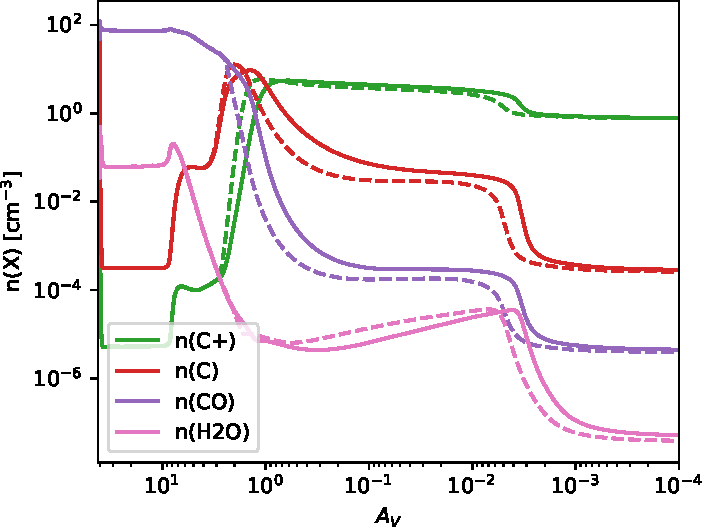
\includegraphics[width=.48\textwidth,keepaspectratio]{cmpH2rt_CO_H2O.pdf}
    \caption{Comparison of temperature profile and abundances for models computed with exact radiative transfer (solid lines) and FGK approximation (dashed lines) for \ce{H2} UV lines: \ce{H} species and \ce{O} (left), and \ce{C}, \ce{CO}, and \ce{H2O} (right).} \label{fig:cmpH2rt}
\end{figure}

\subsubsection{Models with Surface Chemistry} \label{sec:surfchem}
\qt{to consider Emeric's comment?}
In the ISM, direct gas-phase formation of molecules is inefficient for some molecules. Instead, molecules are formed on the surfaces of dust grains, which act as catalysts by providing a surface for adsorbed atoms to meet and react. The grains also absorb the excess energy released by the formation process, preventing dissociation that would otherwise occur in the gas-phase formation. The formation of \ce{H2} is a key demonstration of the importance of this process, as the gas-phase formation rate of \ce{H2} is much lower than the rate required to explain the observed abundance of \ce{H2} in the ISM \parencite{Gould1963,Hollenbach1971}. In addition to chemical reactions, dust grains also play a role in the sublimation and freeze-out of molecules, leading to the sudden apparition or disparition of some molecules at depths where the dust temperature crosses specific threshold values \parencite{Herbst2009}.

\begin{figure}[hb]
    \centering
    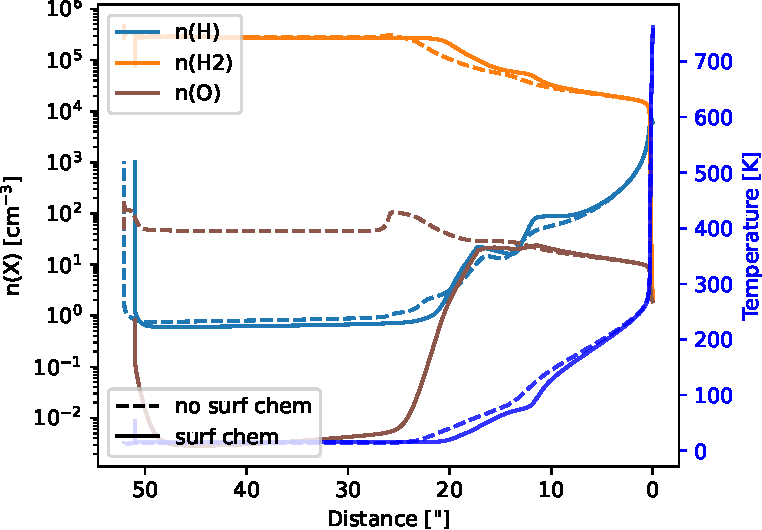
\includegraphics[width=.52\textwidth,keepaspectratio]{cmpsurfb_H_O.pdf}
    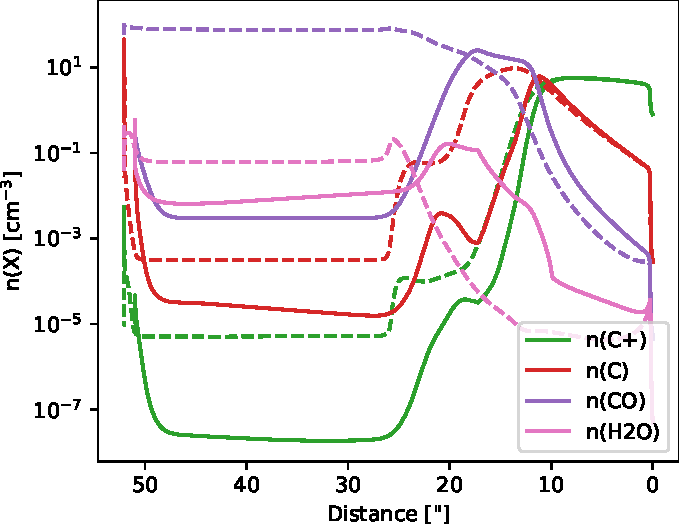
\includegraphics[width=.47\textwidth,keepaspectratio]{cmpsurfb_CO_H2O.pdf}
    \caption{Comparison of temperature profile and abundances for models computed with (solid lines) and without (dashed lines) surface chemistry: \ce{H} species and \ce{O} (left), and \ce{C}, \ce{CO}, and \ce{H2O} (right).} \label{fig:cmpsurfb}
\end{figure}

In Fig.~\ref{fig:cmpsurfb}, I compare the PDR models computed with and without surface chemistry. As previously noted, \ce{H2} formation on grains is by default included in both models. The inclusion of surface reactions leads to a substantial earlier rise in the abundances of $n(\ce{CO})$ and $n(\ce{H2O})$ due to enhanced production on dust grain surfaces. At greater depths within the cloud, the abundances of almost all molecules decrease in the model with surface chemistry because of the freeze-out of molecules onto the dust grains. Grains also reduce the gas temperature, as the abundances of key coolants, such as \ce{CO} and \ce{H2O}, increases, as shown in the left panel. Since \ce{CO} and \ce{H2O} are present in the observations we aim to study, it is crucial to include surface chemistry in the models.

% To summarize the model comparisons in this section, I will use the constant pressure model with exact radiative transfer of \ce{H2} and surface chemistry to consider the curvature of the cloud's surface in the following sections.

As a result of the model comparisons in this section, all models run in this project will use a constant pressure prescription, exact radiative transfer for \ce{H2} UV lines, and surface chemistry.

% \subsection{Modeling Column Densities in Spherical Geometry} \label{sec:sphere}
\subsection{Modeling Column Densities in a Spherical PDR} \label{sec:sphere}
% \begin{wrapfigure}{r}{.32\textwidth}
%     \centering
%     \includegraphics[width=.25\textwidth]{sphere_geometry_2LoS.pdf}
%     \caption{Scheme of the spherical, plane-parallel geometry. Curvature exaggerated for clarity.} \label{fig:geometry}
% \end{wrapfigure}

% \begin{figure}
%     \centering
%     \raisebox{-0.5\height}{\includegraphics[width=.69\textwidth,keepaspectratio]{figures/slab_geometry.png}}
%     \hfill
%     \raisebox{-0.5\height}{\includegraphics[width=.24\textwidth,keepaspectratio]{figures/sphere_geometry_2LoS.pdf}}
%     \caption{Left: scheme of the slab geometry of the \mdpdr{}. Reprinted from \textcite{LePetit2006} Right: scheme of the plane-parallel geometry of the PDR wrapper.} \label{fig:geometry}
% \end{figure}

\begin{figure}
    \centering
    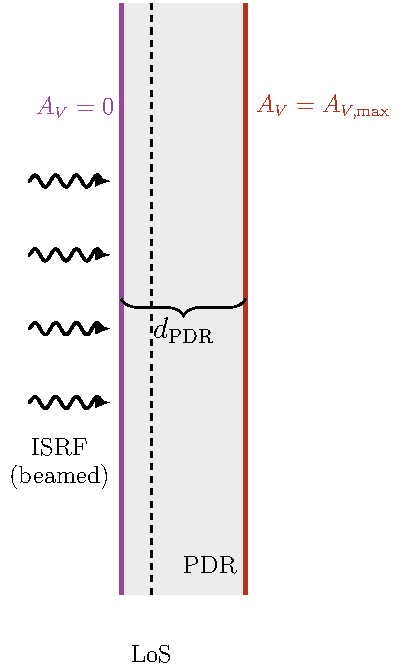
\includegraphics[width=.3\textwidth,height=.35\textheight,keepaspectratio]{slab_geometry.pdf}
    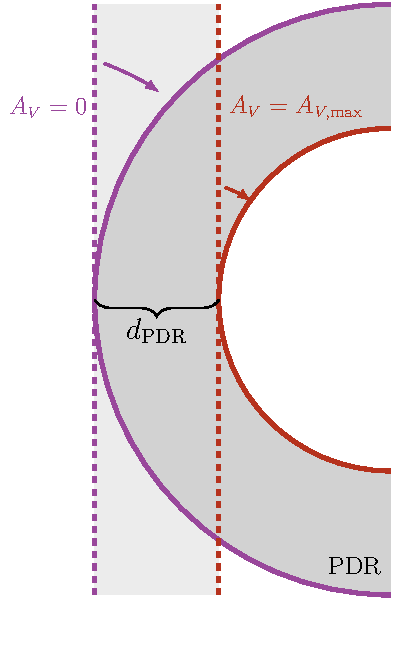
\includegraphics[width=.32\textwidth,height=.35\textheight,keepaspectratio]{slab_to_sphere.pdf}
    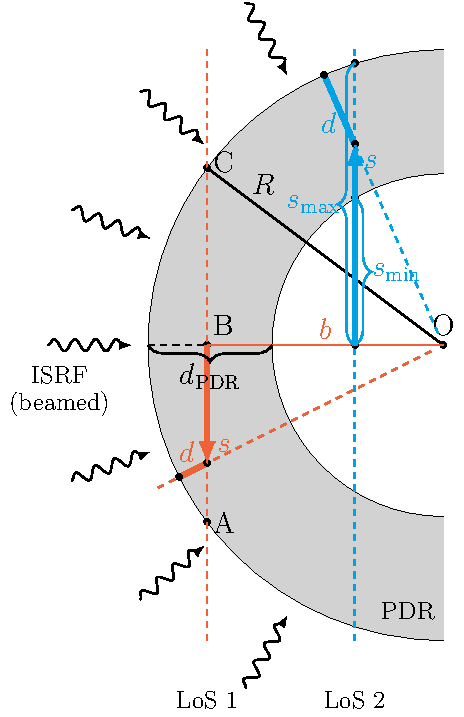
\includegraphics[width=.36\textwidth,height=.35\textheight,keepaspectratio]{sphere_geometry.pdf}
    \caption{Scheme of the slab geometry in \mdpdr{} (left), the transformation from slab to spherical geometry (middle), and the spherical PDR layer with the definition of the different distances used in the text (right). The purple line represents the illuminated front of the PDR, while the red line represents the backside. When transforming from slab geometry to spherical geometry, the beamed ISRF remains perpendicular to the surface. The curvature is exaggerated for clarity.} \label{fig:geometry}
\end{figure}

To model the curvature of the cloud, I treat the PDR as the outermost shell of a fictitious spherical cloud, as illustrated in Fig.~\ref{fig:geometry}. The radial profile of this PDR layer is approximated by the results of a 1D plane-parallel PDR model. This approximation is valid when the depth of the PDR is relatively small compared to the radius of the cloud. For the models in this study, the physical depth of the PDR is approximately $\qty{0.08}{pc}$, which is significantly smaller than the curvature radius, as seen in Fig.~\ref{fig:obsimg}, thereby justifying the use of the plane-parallel approximation. Consequently, all physical variables at a given distance from the cloud's surface are considered as equivalent to those computed by the \mintinline{python}{MeudonPDR} model at the same distance from the cloud's edge.

The radius $R$ of the fictitious spherical cloud is provided as an input parameter to the wrapper code. A LoS is defined by its impact parameter $b$, which measures the perpendicular distance from the LoS to the center of the cloud. From the output of the \mdpdr{}, the level number densities $n_X(d)$ are obtained as a function of the depth $d$ into the cloud. In plane-parallel geometry, $n_X(d)$ gives the number density at a point located at a depth $d$ from the spherical surface. 

The column density along a given LoS is determined by interpolating the number density at any depth $d$ and then integrating along the LoS. To do this, I first compute the range of distances inside the PDR region along the LoS. The maximum half-distance $s_{\max}$ is given by:
\begin{equation}
    s_{\max} = \sqrt{R^2 - b^2},
\end{equation}
while the computation of the minimum half-distance $s_{\min}$ depends on whether the LoS penetrates beyond the PDR region (see the right panel of Fig.~\ref{fig:geometry}):
\begin{equation}
    s_{\min} = \left\{\begin{array}{ll}
       0  &  \text{ if } b > R - d_\mr{PDR}, \text{ LoS 1} \\
       \sqrt{(R - d_\mr{PDR})^2 - b^2}  &  \text{ if } b < R - d_\mr{PDR}, \text{ LoS 2}
    \end{array}\right.,
\end{equation}
where $d_\mr{PDR}$ is the depth of the PDR region. Next, the distance $s$ along the LoS is converted into the depth $d$ from the cloud's surface. Using Pythagorean theorem, one can easily establish that $d = R - \sqrt{s^2 + b^2}$. The number density at each point along the LoS is then calculated as:
\begin{equation}
    n_X(s) = f(R - \sqrt{s^2 + b^2}),
\end{equation}
where $f(d)$ is the interpolated function of the level number density $n_X(d)$. Finally, the column density $N_X(b)$ for a given LoS with impact parameter $b$ is obtained by integrating the number density along the LoS. By symmetry, the total column density is twice the integral over the half-LoS: 
\begin{equation}
    N_X(b) = 2\int_{s_{\min}}^{s_{\max}} n_X(s') \dd{s'}.
\end{equation}
By considering the curvature of the cloud's surface, this column density allows for a more direct comparison with observations. However, this approach does not account for the absorption processes occurring inside the cloud. For lines that are optically thick, the radiative transfer equation must be solved along the LoS to accurately reproduce the observed line profiles. This more detailed treatment will be addressed in the next section.

\subsection{Solving the Radiative Transfer Equation} \label{sec:rte}
The column densities are useful when the lines are optically thin, as they are proportional to the line intensities in this case. However, some lines can be optically thick, leading to differences in the observed spatial profiles for various lines, as seen in Fig.~\ref{fig:observation}. In such cases, a more detailed treatment is required to account for line reabsorption within the cloud. To achieve this, I need to solve the radiative transfer equation along the LoS \parencite[see, e.g.,][ Eq.~1.67]{Rybicki1979}:
\begin{equation}
    \fird[I_\nu]{s} = A_{ul} n_u\frac{h\nu}{4\pi}\phi(\nu) +  B_{ul} n_u\frac{h\nu}{4\pi}I_\nu \phi(\nu) -  B_{lu} n_l\frac{h\nu}{4\pi}I_\nu \phi(\nu), \label{eq:rte}
\end{equation}  
where $n_u$ and $n_l$ are the number densities of the upper and lower levels of the transition, respectively, $h$ is the Planck's constant, $\nu$ is the frequency of the transition, and $\phi(\nu)$ is the line profile. I assume that the line profile is dominated by turbulent broadening, with a constant turbulent velocity dispersion throughout the cloud. Dust is neglected, as its cross sections are relatively low in the far-infrared (FIR) and submillimeter domains.

% The line profile is usually always the same for absorption and emission as it is the same species emitting and absorbing. The approximation here, is that in general the line profile could vary spatially with the position along the line of sight. In particular, it should depend on gas temperature due to thermal broadening, and the temperature does vary with position in the PDR. Here we assume that the line profile are dominated by turbulent broadening and the turbulent velocity dispersion is constant in the cloud.

The coefficients $A_{ul}, B_{ul}, B_{lu}$ in Eq.~\ref{eq:rte} are the Einstein coefficients for spontaneous emission, stimulated emission, and absorption, respectively. These coefficients are intrinsic properties of the specific transition and are related through the Einstein relations \parencite{Einstein1917}:
\begin{equation}
    B_{ul} = \frac{c^2}{2 h \nu_{ul}^3} A_{ul},\, g_l B_{lu} = g_u B_{ul},
\end{equation}
where $g_u$ and $g_l$ are the degeneracies of the upper and lower levels.

In PDRs, the motion of atoms and molecules results in line broadening. Thermal motion produces a Gaussian profile, while microturbulent motions contribute an additional broadening component. The thermal and turbulent broadening effects are combined in the effective Doppler width, $\Delta \nu_D$, which is then included in the Gaussian line profile \parencite[see, e.g.,][Eqs.~10.68-10.72]{Rybicki1979}:
\begin{equation}
    \phi(\nu) = \frac{1}{\sigma_\nu \sqrt{2 \pi}}\exp\left(-\frac{(\nu - \nu_0)^2}{2 \sigma_\nu^2}\right),
\end{equation}
where
\begin{equation}
    \sigma_\nu = \frac{\sqrt{2}}{2}\Delta \nu_D, \quad \Delta \nu_D = \frac{\nu_0}{c}\sqrt{\frac{2 k T}{m} + v_\mr{turb}^2}.
\end{equation}
Here, $\nu_0$ is the central frequency of the transition, $c$ is the speed of light, $T$ is the gas temperature, $m$ is the mass of the emitting species, and $v_\mr{turb} = \qty{2}{\km\per\second}$ is the turbulent velocity, as introduced in Table.~\ref{tab:params}.

The line profile is normalized so that $\int_0^{\infty} \phi(\nu) \dd{\nu} = 1$. To ensure computational efficiency while maintaining a good representation of the profile, I truncate the line profile at $5\sigma$. Therefore, in practice, the normalization becomes $\int_{\nu_0 - 5\sigma}^{\nu_0 + 5\sigma}\phi(\nu) \dd{\nu} = 1$.

% To solve the radiative transfer equation, I also need a background intensity $I_0$. For this, I use the isotropic specific intensity on the observer side, as provided by the \mdpdr{} in the file \mintinline{python}{_IncRadField.dat}. It is important to note that the current implementation is valid only for isotropic radiation; handling more general forms of background specific intensity would require additional modifications. %\qt{add explanation why?} 

To solve the radiative transfer equation, I also need a background intensity $I_0$. In the PDR model, the external radiation field includes a component from the IR/FIR due to dust emission from the surroundings of the PDR. I use this as the background intensity for the radiative transfer calculation.

The external radiation field in the \mintinline{python}{IncRadField.dat} file is provided in units of \unit{erg\per\centi\meter\squared\per\second\per\steradian\per\AA}. However, to solve the radiative transfer equation, I need the specific intensity in units of \unit{erg\per\centi\meter\squared\per\second\per\steradian\per\Hz}. By energy conservation, $I_\nu |\dd{\nu}| = I_\lambda |\dd{\lambda}|$, and using $c = \lambda\nu$, I can derive the differential relation $\dd{\lambda} = -c/\nu^2 \dd{\nu}$. This allows me to convert between the two quantities as follows:
\begin{equation}
    I_\nu = I_\lambda \left|\frac{\dd{\lambda}}{\dd{\nu}}\right| = I_\lambda \frac{c}{\nu^2} = I_\lambda \frac{\lambda^2}{c}.
\end{equation}

Thus far, I have focused on improving the geometry of PDR models. However, the observed spectra are inevitably influenced by the resolution of the instrument used for observation. The instrumental resolution smooths out the line spatial profile, broadening the observed lines and altering their shapes. Consequently, it is essential to account for the instrument's resolution in the modeling process. In the following section, I will discuss the convolution process and how it modifies the observed spectra.

\subsection{Convolution of Line Profiles with Instrumental Resolution} \label{sec:convolution}

The spatial resolution of an instrument is typically characterized by its point spread function (PSF), which describes the response of the instrument to a point source. To account for the effects of instrumental resolution on the observed line profiles, I convolve the model's line profile with the PSF. Since the spatial grid provided by \mdpdr{} is non-uniform, I first interpolate it onto a uniform and monotonic grid.

The PSF is often approximated as a Gaussian function. For this work, the Gaussian kernel is expressed as:
\begin{equation}
    g(x) = \frac{1}{\sigma\sqrt{2\pi}}\exp(-\frac{x^2}{2\sigma^2}),
\end{equation}
where $x$ is the distance from the center of the PSF, and $\sigma$ is the standard deviation of the Gaussian. The standard deviation $\sigma$ is related to the full width half maximum (FWHM) of the instrument by $\sigma = \text{FWHM}\,/\,(2\sqrt{2 \ln 2})$.

To reduce computational cost, I truncate the Gaussian PSF at $3\sigma$, as the contribution from points beyond this range is negligible. The PSF is then normalized over the truncated range to conserve total intensity, with the normalization constant $K = \sum_{x=-3\sigma}^{3\sigma} g(x) \Delta x$, where $\Delta x$ is the spacing of the uniform grid.

The convolution of the line profile, $f(x)$, with the normalized PSF is performed as:
\begin{equation}
    (f * g) (x) = \frac{1}{K} \sum_{\tau = x_{\min} - 3\sigma}^{x_{\max} + 3\sigma}F(\tau)g(x - \tau)\Delta x,
\end{equation}
where $x_{\min}$ and $x_{\max}$ define the bounds of the spatial grid, and $F(\tau)$ is the value of the line profile at point $\tau$. Illustrations of the effects of convolution on line profiles can be found in Figs.~\ref{fig:convolution_surfchem} and \ref{fig:convolution_nosurfchem} in the appendix. With increasing FWHM, the convolved profiles become progressively smoother; the peak intensity decreases, and the signal is redistributed over a broader spatial range.

% Fig.~\ref{fig:convolution} \qt{or Fig.~\ref{fig:convolution_nosurfchem}?} illustrates how convolution alters the line profile. The convolved profiles demonstrate how increasing the FWHM progressively smooths the line profile, reducing peak intensity and redistributing the signal over a broader spatial range.

% \begin{figure}[h]
%     \centering
%     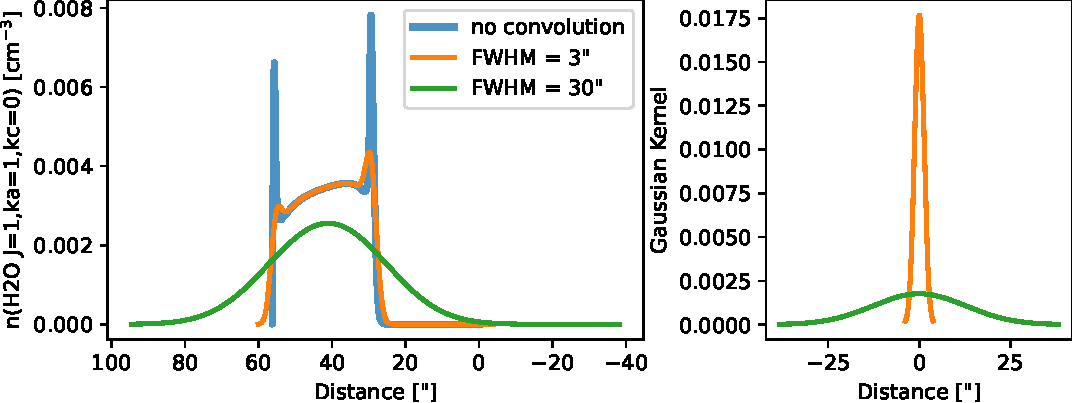
\includegraphics[width=.88\textwidth,keepaspectratio]{convolution_nosurfchem.pdf}
%     \caption{Illustration of the Convolution Process. The left panel shows the original line profile (blue) alongside the profiles convolved with Gaussian PSFs of resolutions $3''$ (orange) and $30''$ (green). The right panel shows the corresponding Gaussian PSFs, normalized and truncated at $3\sigma$.} \label{fig:convolution_nosurfchem}
% \end{figure}

% \begin{figure}[h]
%     \centering
%     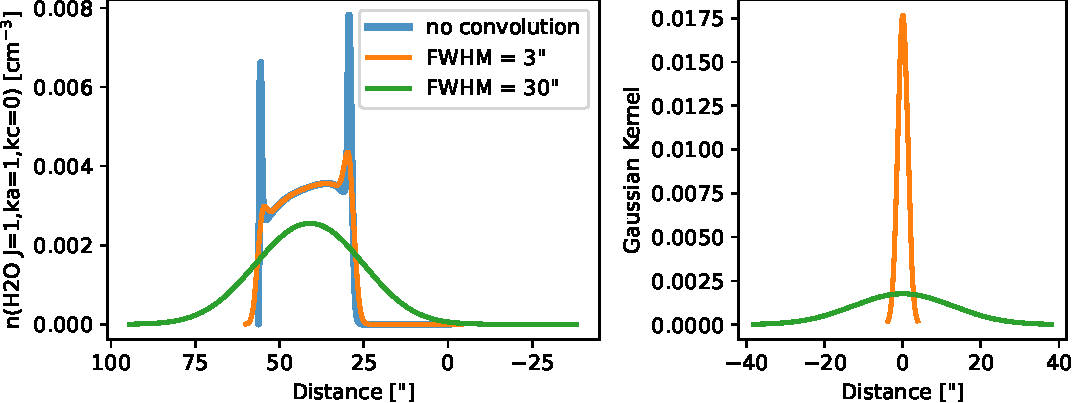
\includegraphics[width=.88\textwidth,keepaspectratio]{convolution.pdf}
%     \caption{Illustration of the Convolution Process. The left panel shows the original line profile (blue) alongside the profiles convolved with Gaussian PSFs of resolutions $3''$ (orange) and $30''$ (green), with a zoomed-in view of the area within the dashed rectangle. The right panel shows the corresponding Gaussian PSFs, normalized and truncated at $3\sigma$.} \label{fig:convolution}
% \end{figure}

\section{Results and Discussion} \label{sec:results}
\subsection{Convolved Column Densities from Spherical Model} \label{sec:convcolden}

\begin{figure}
    \centering
    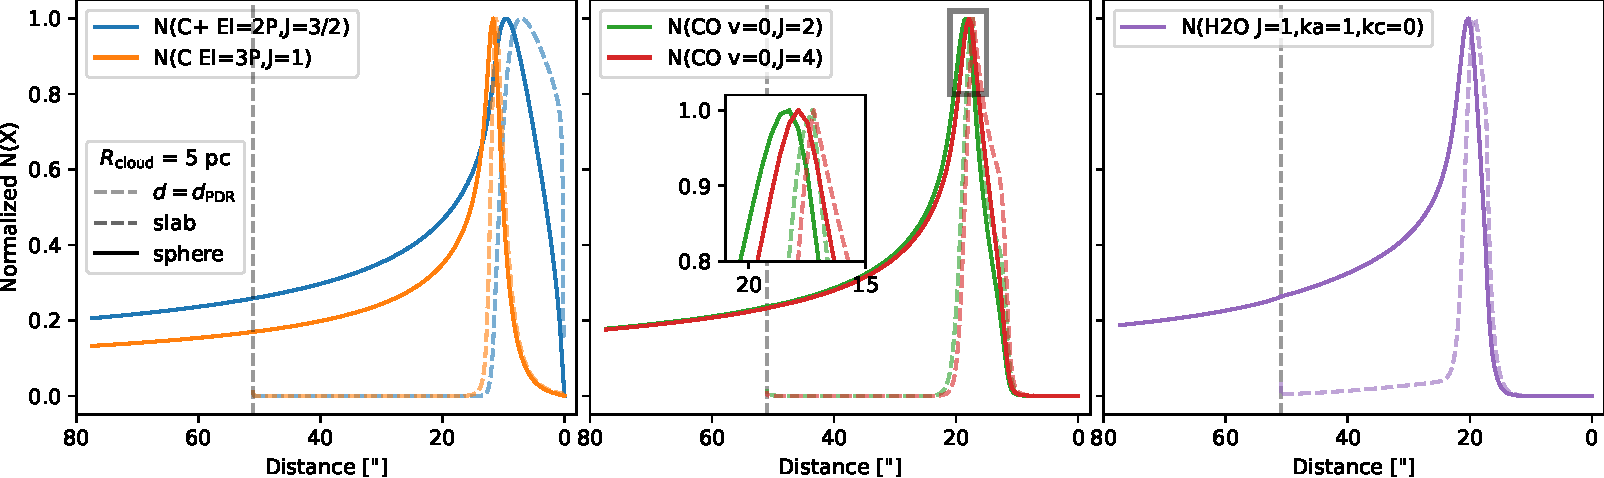
\includegraphics[width=\textwidth,keepaspectratio]{column_densities.pdf} 
    \caption{Comparison of normalized column density profiles for slab geometry (dashed lines) and spherical geometry (solid lines) with a cloud radius \( R_\mr{cloud} = \qty{5}{pc} \). Panel 1: \( N(\ce{C^+}\ \text{2P, J=3/2}) \) (blue) and \( N(\ce{C}\ \text{3P, J=1}) \) (orange). Panel 2: \( N(\ce{CO}\ \text{v=0, J=2}) \) (green) and \( N(\ce{CO}\ \text{v=0, J=4}) \) (red). Panel 3: \( N(\ce{H2O}\ \text{J=1, ka=1, kc=0}) \) (purple). Dashed gray lines indicate the maximum depth of the PDR model,  $d_\mr{PDR}$. The rectangle marks the zoomed-in region in Panel 2.} \label{fig:colden}  
\end{figure}

In Secs.~\ref{sec:sphere} and \ref{sec:convolution}, I described the modeling of spherical geometry using the wrapper for the \mdpdr{} and the convolution of line profiles with the instrumental resolution. In this section, I present the convolved column density profiles for the spherical geometry model with a cloud radius of $R_\mr{cloud} = \qty{5}{pc}$. Comparisons are made first between the spherical and slab geometry models, then between the unconvolved and convolved profiles, and finally between the convolved profiles and the observational data.

Fig.~\ref{fig:colden} compares the profiles from the spherical geometry model with those from the slab geometry models. In the spherical geometry model, the curvature of the cloud's surface causes the PDR layer to bend away from the tangent at the cloud's surface, in contrast to the slab geometry, where the PDR layer is directly at the surface. As a result, the PDR layer reaches greater depths in the spherical geometry, producing a more extended profile. Additionally, the peaks shift to deeper locations within the cloud, as the line of sight (LoS) passing through the greatest distance within the emitting region is slightly behind the emitting region. When convolution with instrument resolution is applied, the line profiles are smoothed and further extended (Fig.~\ref{fig:convvcolden}), with the peaks shifting to greater depths. The convex tail behind the emitting region disappears, yielding a more Gaussian-like shape. 

The convolved profiles provide a better match to the observed data, as shown in Fig.~\ref{fig:colden_Rcloud5pc}, particularly in terms of the shape and extent of the profiles. The peak widths are relatively consistent with the observations, and with spherical geometry, we begin to observe an asymmetry in the spatial profiles. This suggests that including curvature and convolution improves the modeling of the observed column density profiles. However, except for \ce{C+}, the asymmetry does not align well with the observed profiles. Moreover, the shift between \ce{C+/C} and the earlier peak of \ce{H2O} in the observations are not reproduced by the models. A possible explanation for this discrepancy could be the cloud radius, which is a free parameter in the model. In the following section, I will explore how varying the cloud radius affects the column density profiles.

\begin{figure}
    \centering
    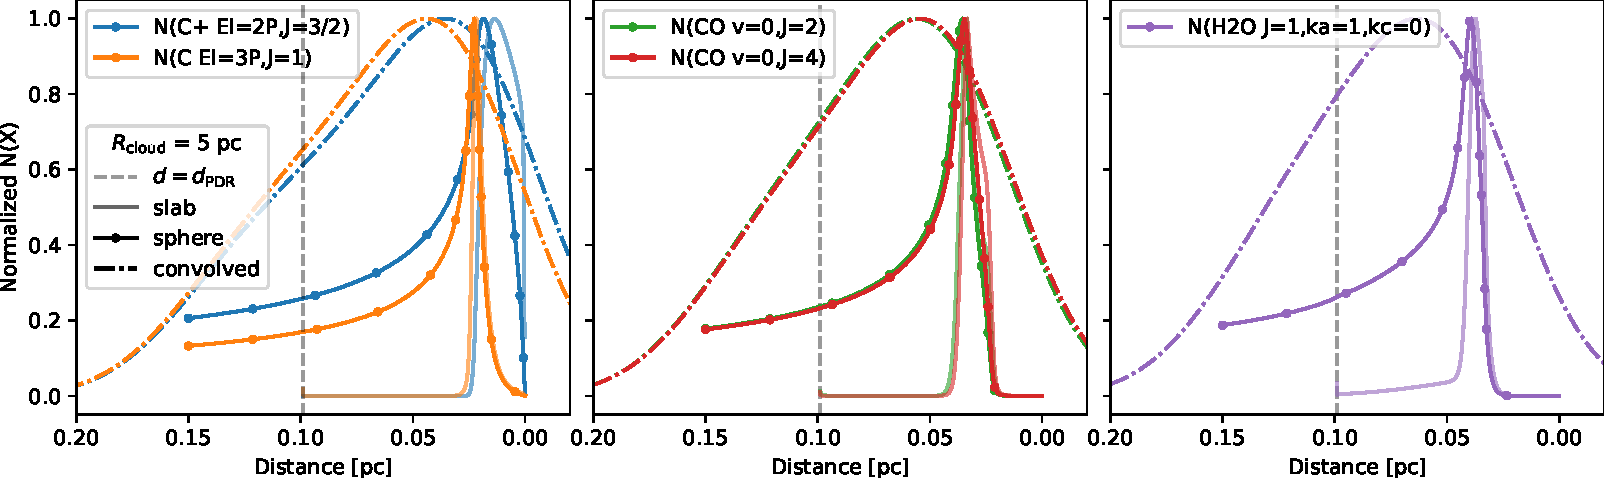
\includegraphics[width=\textwidth,keepaspectratio]{convolved_column_densities.pdf}
    \caption{Similar to Fig.~\ref{fig:colden}, but showing the comparison between unconvolved (dashed lines) and convolved (solid lines) column densities.} \label{fig:convvcolden}
    % \caption{Comparison of normalized column density profiles for slab geometry (solid lines), spherical geometry (solid lines with dots) with a cloud radius of $R_\mr{cloud} = \qty{5}{pc}$, and spherical geometry convolved with the instrument FWHM, $38.1''$. Panel 1 shows $N(\ce{C^+}\ \text{2P, J=3/2})$ (blue) and $N(\ce{C}\ \text{3P, J=1})$ (orange); Panel 2 shows $N(\ce{CO}\ \text{v=0, J=2})$ (green) and $N(\ce{CO}\ \text{v=0, J=4})$ (red); and Panel 3 shows $N(\ce{H2O}\ \text{J=1, ka=1, kc=0})$ (purple). The dashed gray lines indicate the maximum depth of the PDR model, $d_\mr{PDR}$. In spherical geometry, curvature causes the emitting region to appear to extend beyond this depth. Convolution further smooths the line shapes and extends the profiles.} \label{fig:convvcolden}
\end{figure}

\begin{figure}
    \centering
    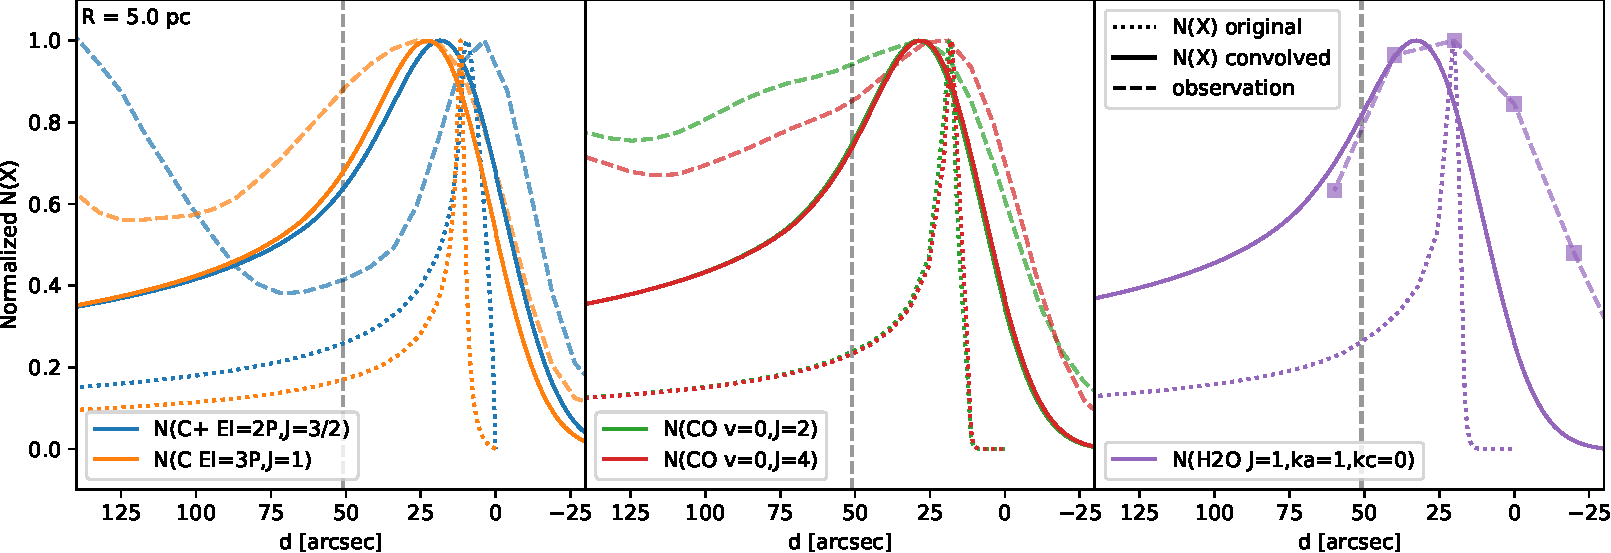
\includegraphics[width=\textwidth,keepaspectratio]{colden_Rcloud5pc.pdf}
    \caption{Comparison of column density profiles for a model with spherical geometry ($R_\mr{cloud} = \qty{5}{pc}$, solid lines) and observations (dashed lines). The unconvolved profiles (dotted lines) are also shown for comparison.} \label{fig:colden_Rcloud5pc}
\end{figure}

\subsection{Effect of Cloud Radius on Column Densities} \label{sec:comprad}

There are no significant changes to the rising side of the profiles or the locations of the peaks with varying cloud radius $R_\mr{cloud}$. Instead, variations in $R_\mr{cloud}$ primarily affect the shape of the profile's tail (Fig.~\ref{fig:comprad}). As the cloud radius increases, the surface curvature decreases, making the emitting region more tangent to the LoS at the same depth from the cloud's surface. This reduces the passage length and, consequently, causes the tail to decline more steeply.

None of the models reproduce the observed profiles accurately. A direct comparison, with profiles overlapped to emphasize differences in shape, is provided in Fig.~\ref{fig:comprad_shape} in the appendix. Notably, the observed profiles exhibit significant variation in the tail shape, whereas the modeled profiles remain quite similar. This discrepancy is likely due to the lack of a detailed treatment of radiative transfer along the LoS, as mentioned in Sec.~\ref{sec:rte}, which I will address in the next section.

\begin{figure}[h]
    \centering
    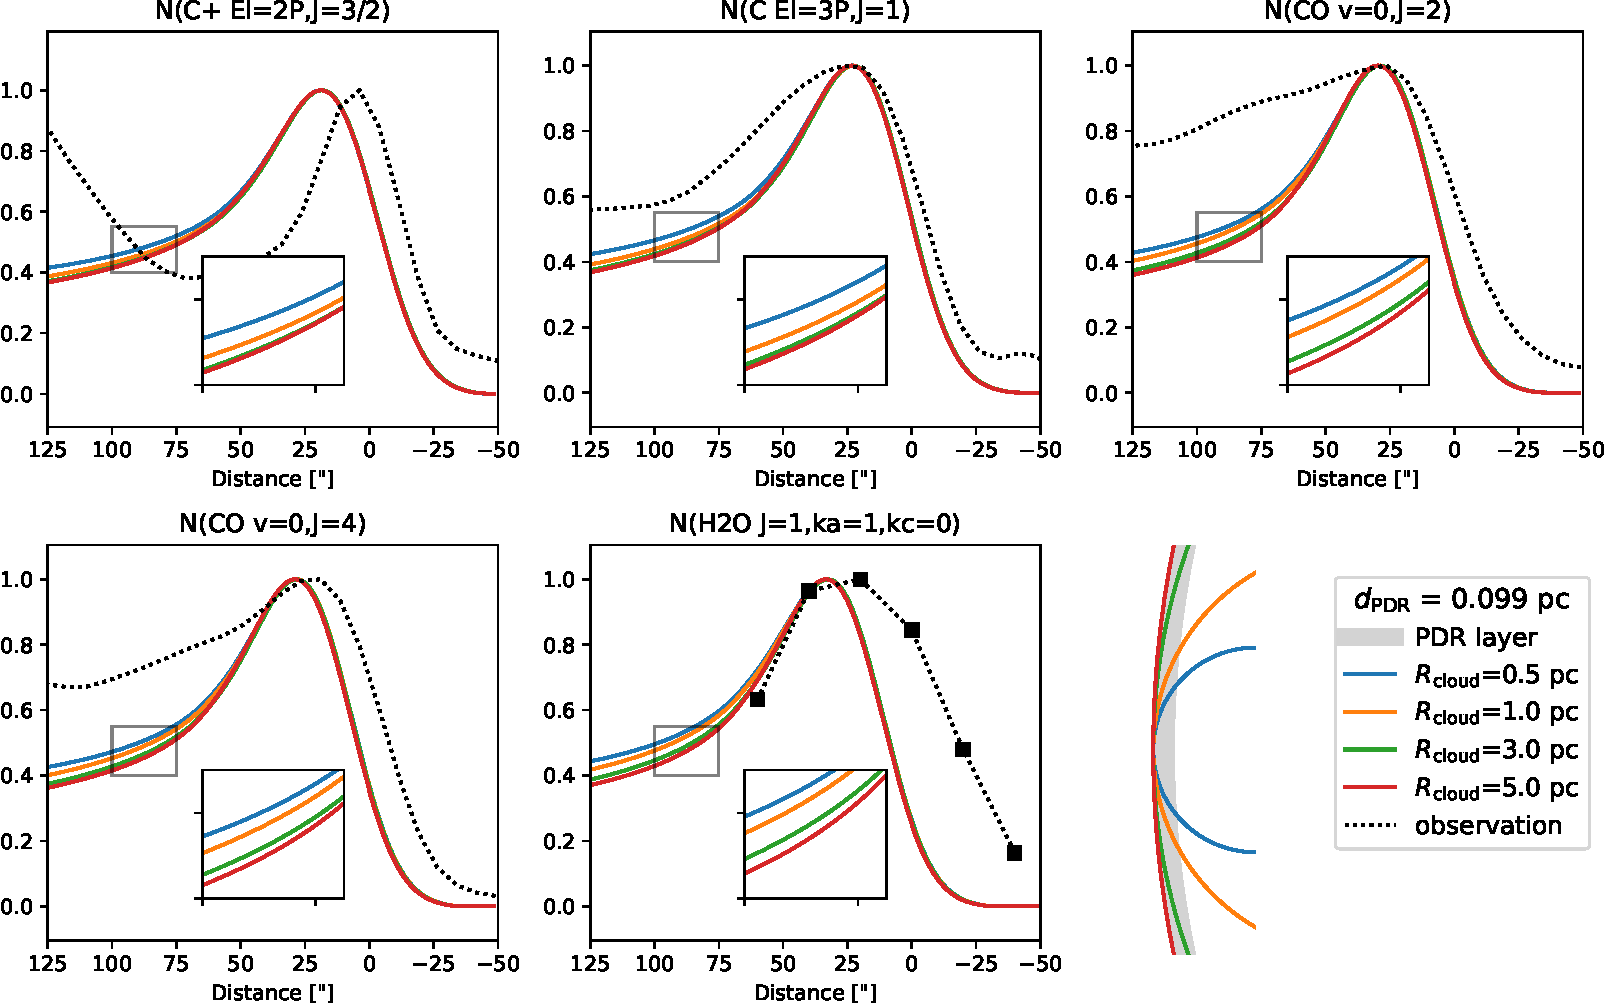
\includegraphics[width=\textwidth,keepaspectratio]{comp_cloud_radius.pdf}
    \caption{Comparison of normalized line profiles for different cloud radii: $R_\mr{cloud} = $ \qty{0.5}{pc} (blue), \qty{1.0}{pc} (orange), \qty{3.0}{pc} (green), and \qty{5.0}{pc} (red). Observations are shown as dotted lines. A schematic representation of the cloud radii is included in the bottom right corner. The areas marked by black rectangles are shown with greater detail in zoomed-in views.} \label{fig:comprad}
\end{figure}

\subsection{Line Profiles with Radiative Transfer} \label{sec:comprte}

To validate the solver, I test it by solving the radiative transfer equation with constant density profiles for both the lower and upper levels, for which an analytical solution can be obtained. In this case, the radiative transfer equation simplifies to:
\begin{equation}
    \fird[I_\nu]{s} = c_1  + c_2 I_\nu, \label{eq:simple_rte}
\end{equation} 
where $c_1 = A_{ul} n_u \phi(\nu) h\nu/4\pi$ and $c_2 = (B_{ul} n_u - B_{lu} n_l) \phi(\nu) h\nu/4\pi$ are constants. The analytical solution to this equation is:
\begin{equation}
    I_\nu (s) = (I_0 + \frac{c_1}{c_2})e^{c_2s} - \frac{c_1}{c_2}.
\end{equation}
For this toy problem, I solve the radiative transfer equation for the \ce{CO} transition from  \(v = 0\), \(J = 2\) to \(v = 0\), \(J = 1\), assuming constant density profiles of $n_u = \qty{2}{\cm^{-3}}$ and $n_l = \qty{2}{\cm^{-3}}$. The computed results are compared with the analytical solution in Fig.~\ref{fig:rtecstn}.

\begin{figure}[h]
    \centering
    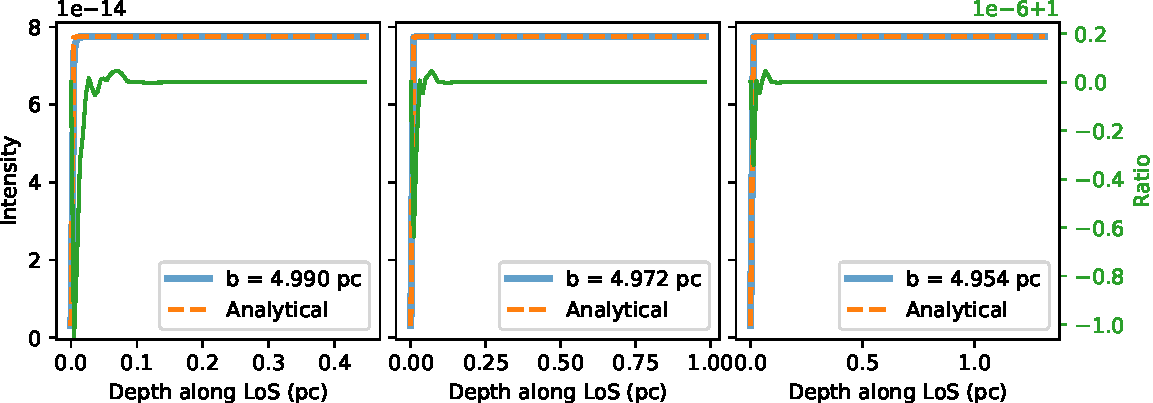
\includegraphics[width=\textwidth,keepaspectratio]{rte_constant_density.pdf}
    \caption{Comparison of the computed (blue solid lines) and analytical (orange dashed lines) solutions to the radiative transfer equation for the \ce{CO} transition from \(v = 0\), \(J = 2\) to \(v = 0\), \(J = 1\) along LoS with different impact parameters in a \(\qty{5}{pc}\) cloud. The right axes show the relative error of the numerical solution, defined as $|I_\nu^\text{num} - I_\nu^\text{ana}|/I_\nu^\text{ana}$.} \label{fig:rtecstn}
\end{figure}

Due to time constraints, I was unable to fully implement the method discussed in Sec.~\ref{sec:rte}. Specifically, my results are limited to solving the radiative transfer equation at the line center, without taking into account the line-broadening profile, $\phi(\nu)$. The preliminary results for the line centers are presented in Fig.~\ref{fig:rtecomp} in the appendix. Despite this limitation, the implemented methods illustrate how solving the radiative transfer equation along the LoS affects the shape of the profiles. Future work could build on these results by incorporating the full line-broadening profile and comparing the results with observed data.

% \begin{figure}
%     \centering
%     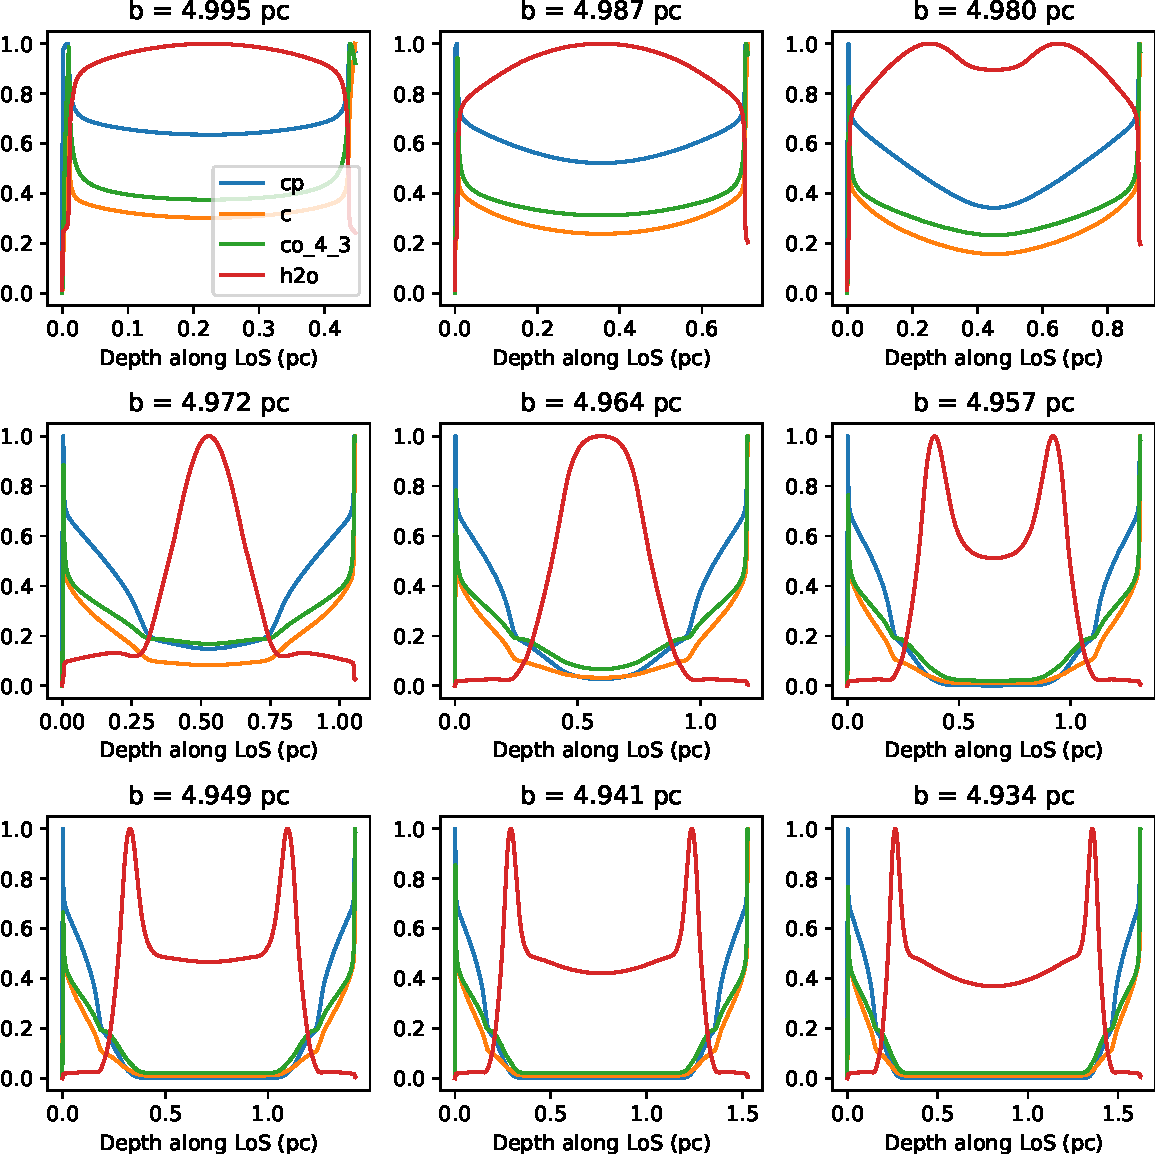
\includegraphics[width=\textwidth,keepaspectratio]{rte_comparison.pdf}
%     \caption{Solution of the radiative transfer equation along LoS with different impact parameters for several lines.} \label{fig:rtecomp}
% \end{figure}

\section{Conclusions} \label{sec:conclusion}

This project developed a wrapper for the \mdpdr{} to compute column densities in spherical geometry and convolve them with the instrumental resolution. The wrapper transforms the output of \mdpdr{}, a 1D slab geometry PDR model, into spherical geometry. Column densities along a given line of sight are derived by interpolating the number densities at various depths and integrating along the line of sight. These column densities are then convolved with the instrumental resolution to account for the effects of the instrument on the observed spatial profiles. 

The convolved column density profiles were compared with observational data of several emission lines along a cut through the Horsehead Nebula. The results show that spherical geometry significantly alters the column density profiles compared to slab geometry, producing more extended profiles with peaks shifted to greater depths within the cloud. Convolution with the instrumental resolution further smooths and extends these profiles, improving their agreement with observed data, particularly in terms of shape and extent. While the peak widths align well with the observations, some discrepancies remain. Specifically, the models fail to capture the shift between \ce{C+/C} and the earlier peak of \ce{H2O}.

The effects of varying the cloud radius on the column density profiles are minimal, primarily influencing the shape of the spatial profile's tail, with little impact on the rising sides or peak locations. As such, adjusting the cloud radius alone cannot resolve the discrepancies.

Preliminary work on solving the radiative transfer equation along the line of sight in spherical geometry is also presented. The comparison between the solution based on \mdpdr{} output and observational data is still ongoing, and further improvements in profile modeling are anticipated with this development.

This work establishes a method for interpreting observational data and determining physical parameters of edge-on PDR observations using models. Future work will focus on refining the radiative transfer treatment and incorporating full line-broadening profiles to further enhance model-observation consistency.

\clearpage
\addcontentsline{toc}{section}{References}
\printbibliography

\clearpage
\appendix
\section*{Supplementary Material}
\addcontentsline{toc}{section}{Supplementary Material}

\subsection*{Comparisons between Constant Pressure and Constant Density Models}
\begin{figure}[h!]
    \centering
    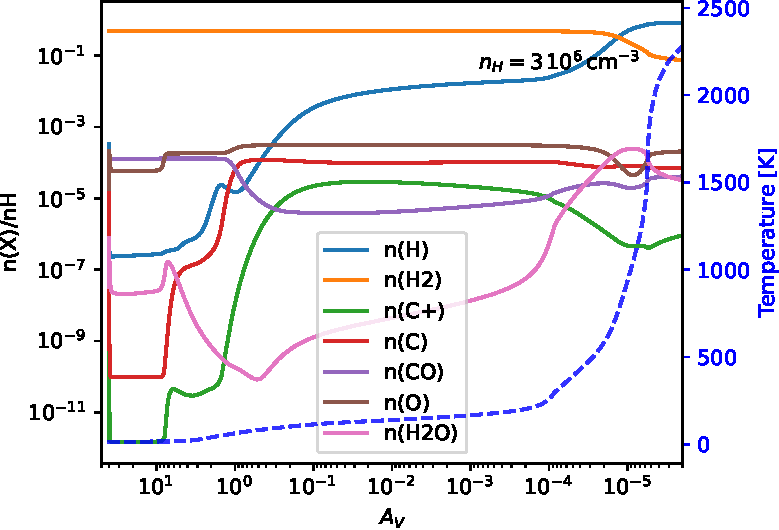
\includegraphics[width=.48\textwidth]{struct_nH3e6.pdf}
    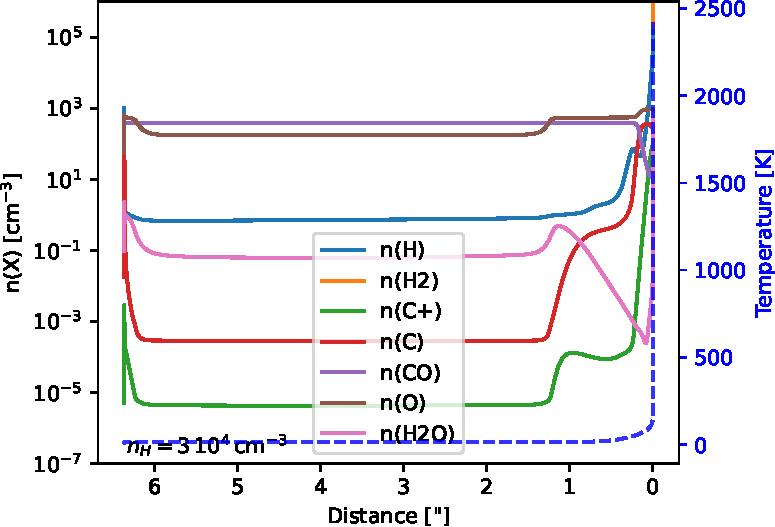
\includegraphics[width=.48\textwidth]{struct_nH3e6_arcsec.pdf}
    \caption{Similar to Figs.~\ref{fig:cmp_cstp_cstn} (left) and \ref{fig:cmp_cstp_cstn_arcsec} (right), for the model with constant density $n_H = \qty{3e6}{cm^{-3}}$.} \label{fig:struct_nH3e6}

    \vspace{2em}

    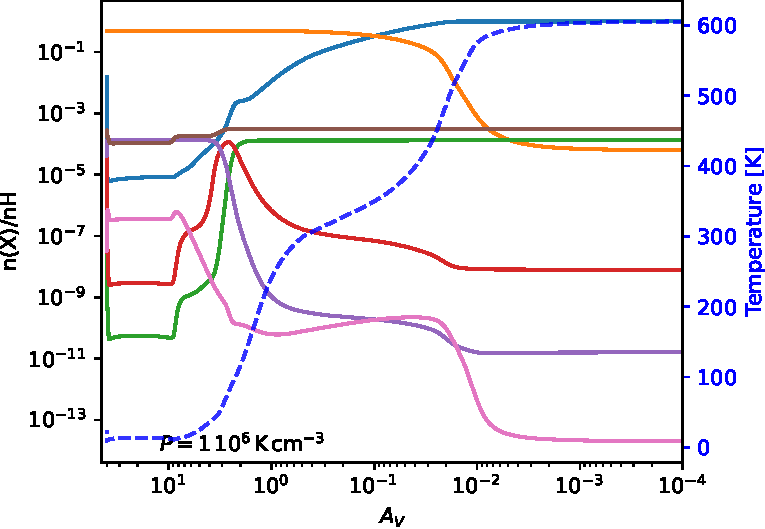
\includegraphics[width=.48\textwidth]{struct_P1e6.pdf}
    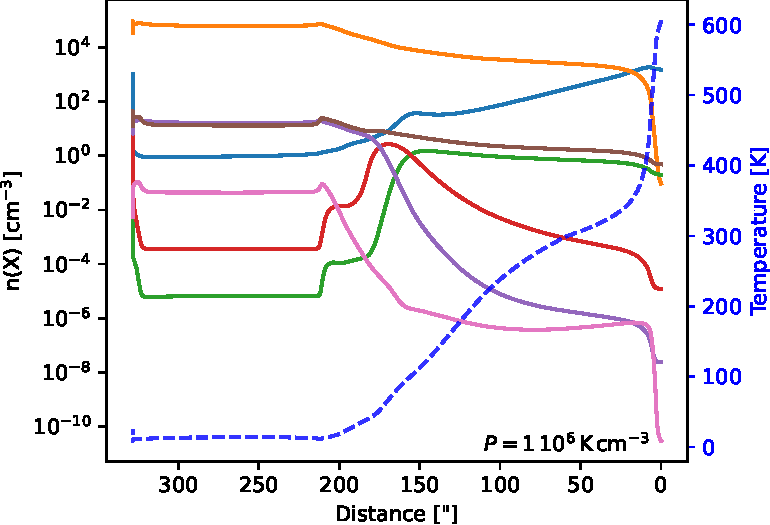
\includegraphics[width=.48\textwidth]{struct_P1e6_arcsec.pdf}
    \caption{Similar to Figs.~\ref{fig:cmp_cstp_cstn} (left) and \ref{fig:cmp_cstp_cstn_arcsec} (right), for the model with constant pressure $P = \qty{1e6}{K\,cm^{-3}}$.} \label{fig:struct_P1e6}

    \vspace{2em}

    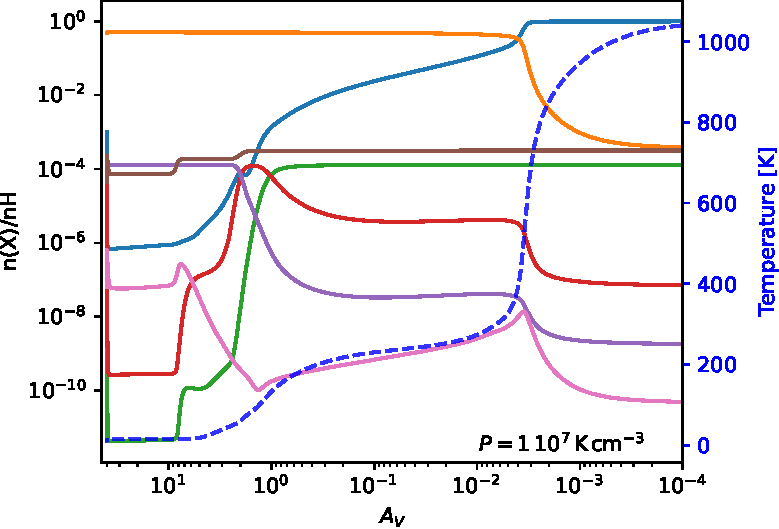
\includegraphics[width=.48\textwidth]{struct_P1e7.pdf}
    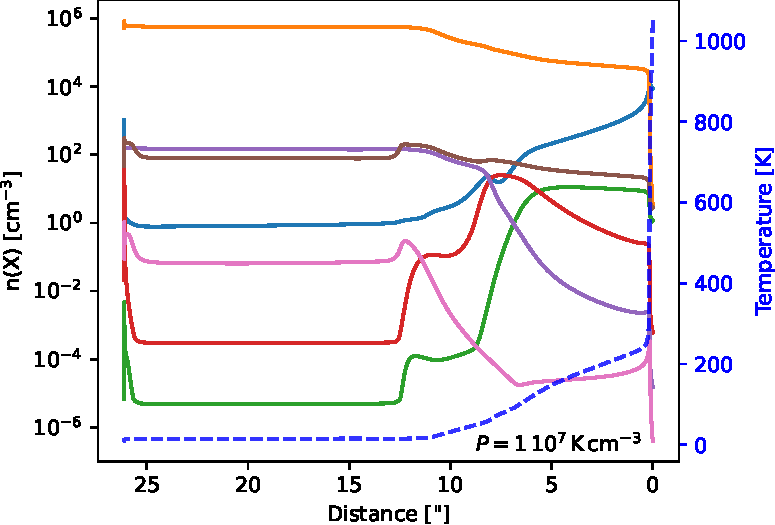
\includegraphics[width=.48\textwidth]{struct_P1e7_arcsec.pdf}
    \caption{Similar to Figs.~\ref{fig:cmp_cstp_cstn} (left) and \ref{fig:cmp_cstp_cstn_arcsec} (right), for the model with constant pressure $P = \qty{1e7}{K\,cm^{-3}}$.} \label{fig:struct_P1e7}

\end{figure}

\clearpage
\subsection*{Convolution}
\begin{figure}[h!]
    \centering
    
    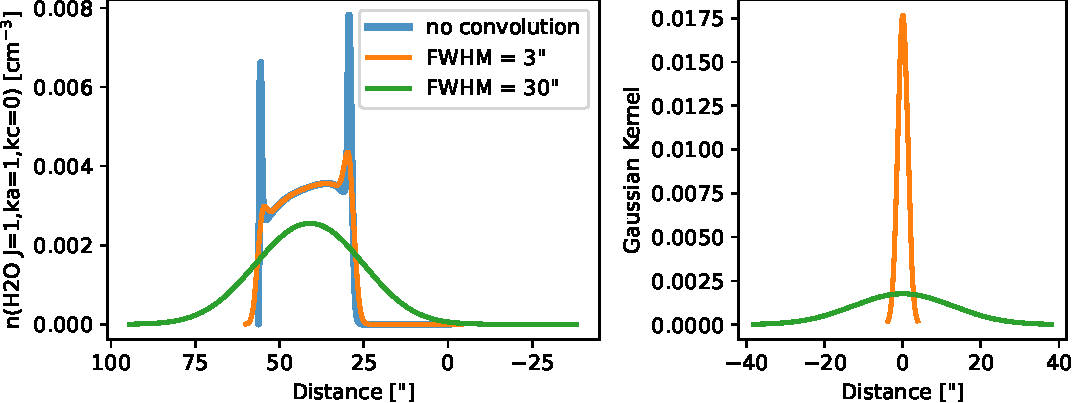
\includegraphics[width=.88\textwidth,keepaspectratio]{convolution.pdf}
    \caption{Illustration of the convolution process using the model with surface chemistry. The left panel shows the original line profile (blue) alongside the profiles convolved with Gaussian PSFs of resolutions $3''$ (orange) and $30''$ (green). The right panel shows the corresponding Gaussian PSFs, normalized and truncated at $3\sigma$.} \label{fig:convolution_surfchem}

    \vspace{2em}

    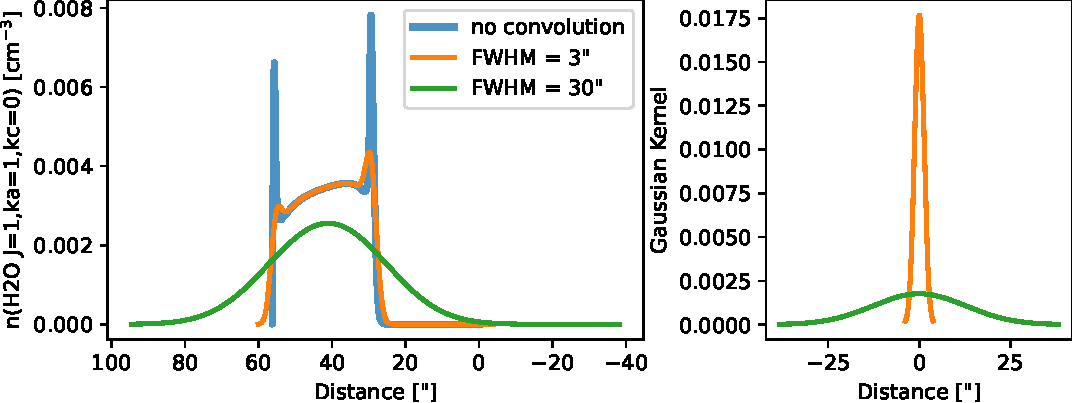
\includegraphics[width=.88\textwidth,keepaspectratio]{convolution_nosurfchem.pdf}
    \caption{Illustration of the convolution process using the model without surface chemistry. The left panel shows the original line profile (blue) alongside the profiles convolved with Gaussian PSFs of resolutions $3''$ (orange) and $30''$ (green). The right panel shows the corresponding Gaussian PSFs, normalized and truncated at $3\sigma$.} \label{fig:convolution_nosurfchem}

\end{figure}

\clearpage
\subsection*{The Effect of Cloud Radius on Column Densities}
\begin{figure}[h!]
    \centering
    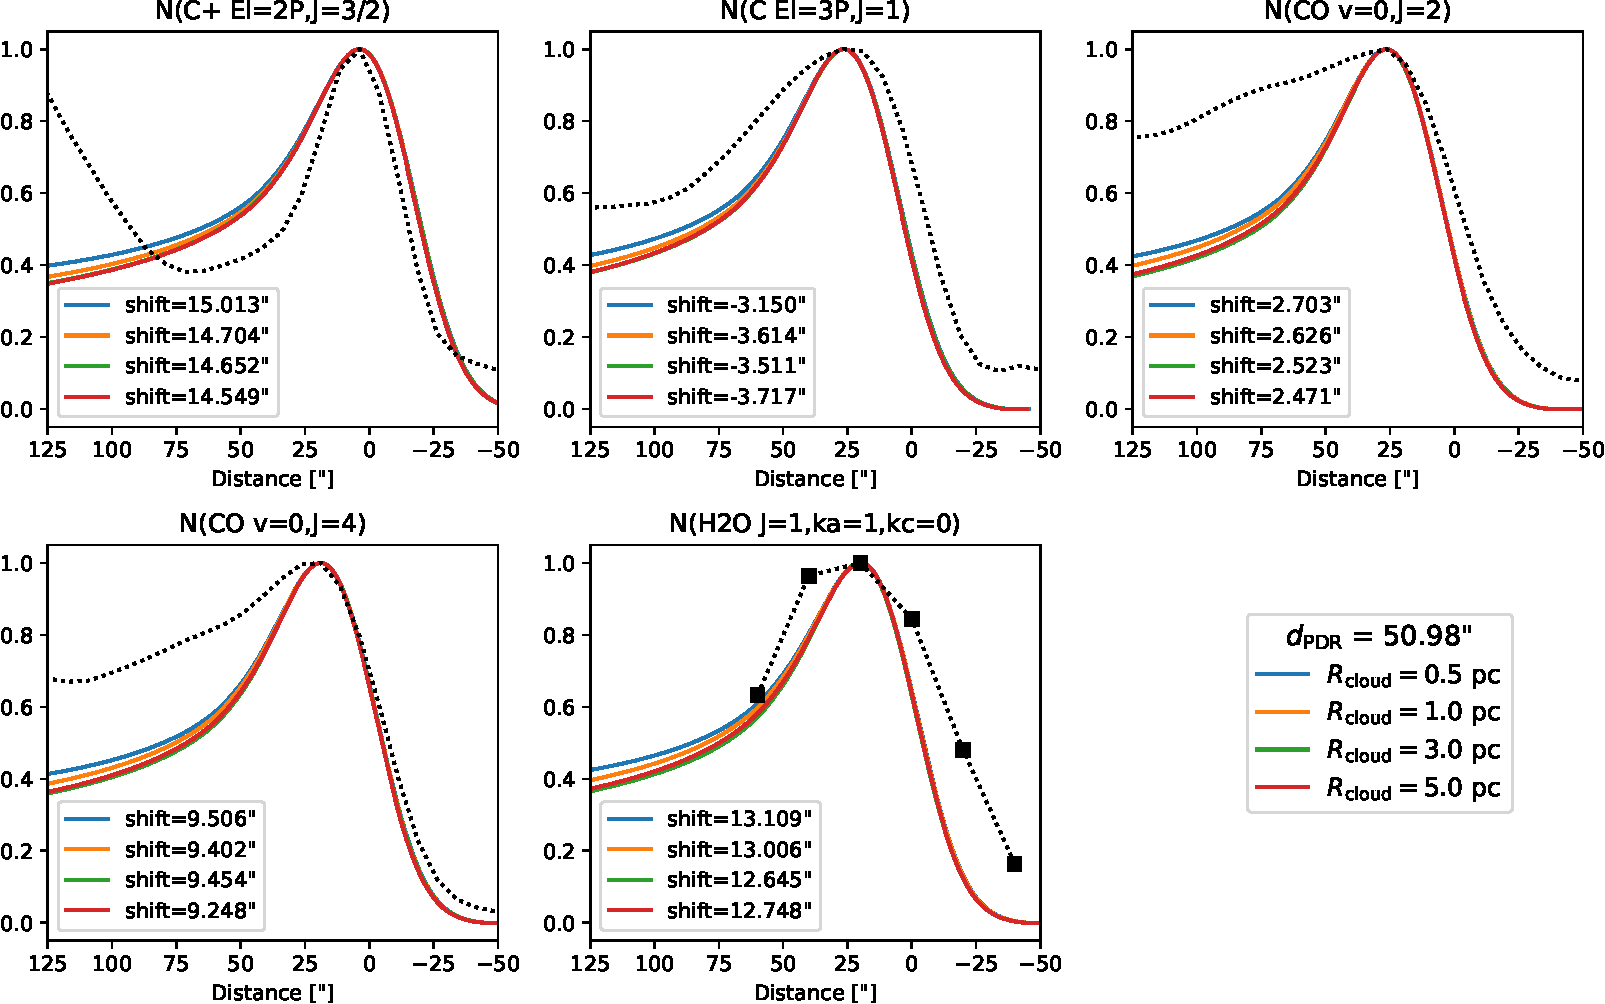
\includegraphics[width=\textwidth,keepaspectratio]{comp_curvature_obs_shape.pdf}
    \caption{Comparison of normalized line profiles for different cloud radii: $R_\mr{cloud} = \qty{0.5}{pc}$ (blue), \qty{1.0}{pc} (orange), \qty{3.0}{pc} (green), and \qty{5.0}{pc} (red). The profiles are shifted to align with the peak locations in the observational data (dotted lines), with the corresponding shifts for each model indicated in the legend.} \label{fig:comprad_shape}
\end{figure}

\clearpage
\subsection*{Solving Radiative Transfer Equation Preliminary Results}
\begin{figure}[h]
    \centering
    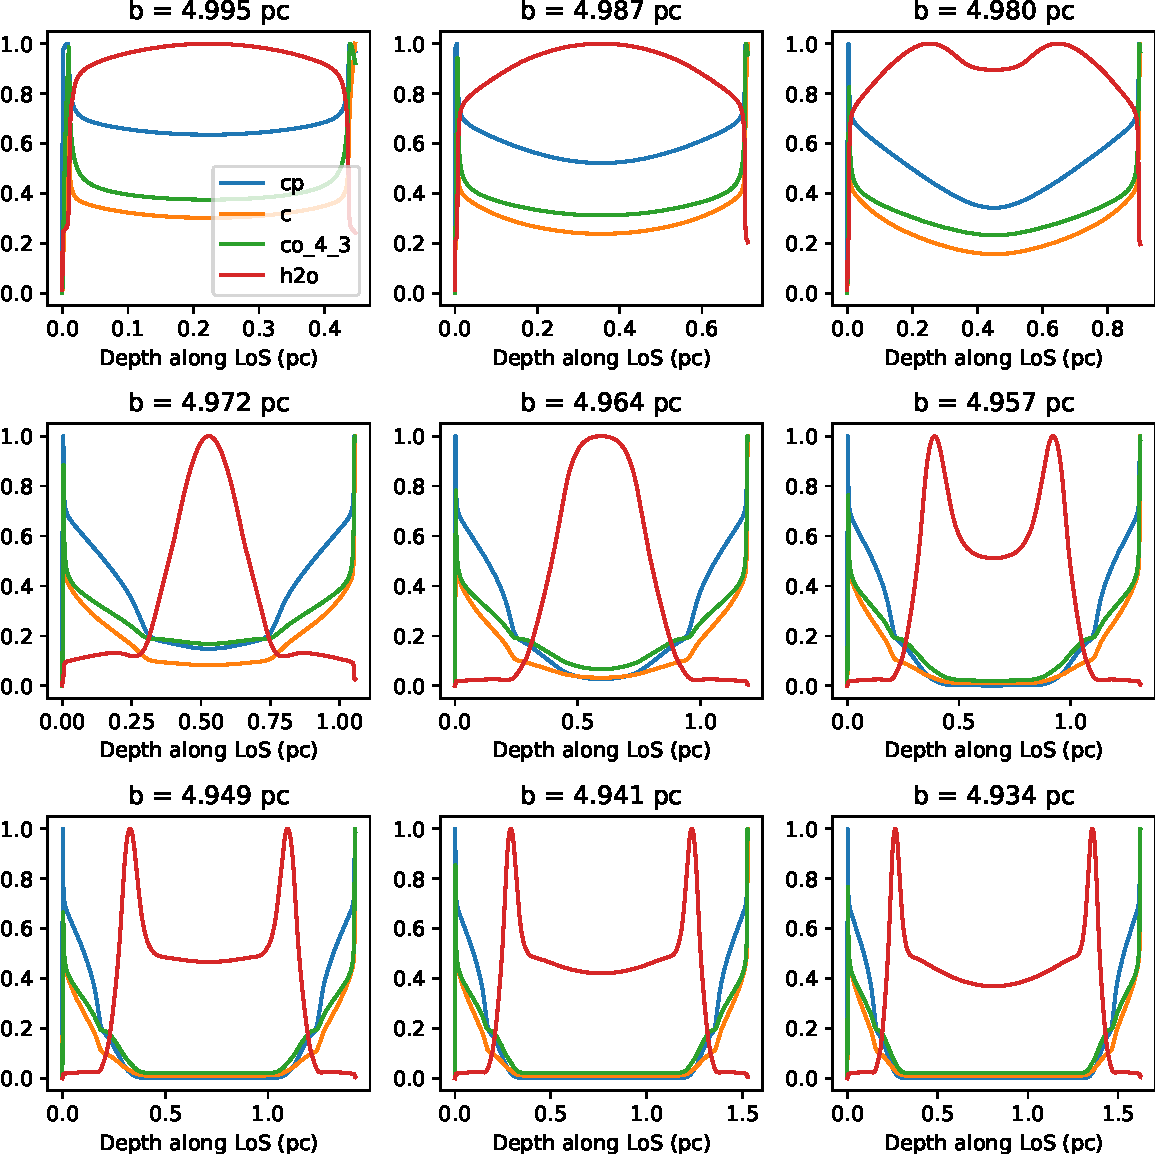
\includegraphics[width=\textwidth,keepaspectratio]{rte_comparison.pdf}
    \caption{Solution of the radiative transfer equation along LoS with different impact parameters for several lines.} \label{fig:rtecomp}
\end{figure}

\end{document}